\documentclass[11pt, a4paper]{article}
%=========================== PACKAGES =============================%

\usepackage[utf8]{inputenc} 
\usepackage[T1]{fontenc} 

\usepackage[hmargin=2.00cm, top=1.8cm, bottom=4.0cm]{geometry}
\usepackage[brazil]{babel} 

\usepackage{longtable}
  
\usepackage{graphicx}
\usepackage{placeins}
\usepackage{subcaption}
\usepackage{float} 

\usepackage{hhline}
\usepackage{courier}
 
\usepackage{amsmath}
\usepackage{bm}
\usepackage{amsfonts}

\usepackage{hyperref}

\usepackage{listings}
\renewcommand\lstlistingname{Programa}
 
 
\usepackage{color} %red, green, blue, yellow, cyan, magenta, black, white
\lstset{language=bash,%
    basicstyle=\footnotesize\ttfamily,
    breaklines=true,%
    keywordstyle=[4]{\color{black}},
    frame= single,
}
 
\lstdefinestyle{nonumbers}
{numbers=none} 

\usepackage{multirow}
\usepackage{float}

\usepackage{enumerate}

\usepackage{fancyhdr}
\pagestyle{fancy} 

\rhead{
\includegraphics[height=1.6cm]{image/CNPEM}}
\lhead{
\includegraphics[height=1.6cm]{image/LNLS}}

\cfoot{\footnotesize O LNLS integra o Centro Nacional de Pesquisa em Energia e
Materiais (CNPEM), Organização Social qualificada pelo Ministério da Ciência,
Tecnologia, Inovações e Comunicações (MCTIC) \\ 
Campus: Rua Giuseppe Máximo Scolfaro, 10.000 - Pólo II de Alta Tecnologia -
Caixa Postal 6192 - 13083-970 - Campinas/SP\\
Fone: +55.19.3512.1010 | Fax: +55.19.3512.1004 | www.lnls.cnpem.br} 
\renewcommand\headrulewidth{0pt}

\usepackage[scaled]{helvet}
\renewcommand\familydefault{\sfdefault} 
\usepackage[T1]{fontenc}

\usepackage{setspace}

\hyphenation{ res-pon-sá-ve-is }
\hyphenation{ cons-tan-te }
\hyphenation{ res-pec-ti-vo }
\hyphenation{ con-fi-gu-ra-mos }
\hyphenation{ fun-ci-o-na-li-da-des }
\hyphenation{ dis-po-ní-veis }

%=========================== PACKAGES =============================%


\author{Gustavo Ciotto Pinton}

\begin{document}

\selectlanguage{brazil}

\begin{center}

\pagenumbering{gobble}

\vspace*{12pt}

LNLS - LABORATÓRIO NACIONAL DE LUZ SÍNCROTRON

\vspace*{.30\textheight}

{\Large GUSTAVO CIOTTO PINTON}

\vspace*{72pt}

\textbf{\Large Desenvolvimento de \textit{Software} e \textit{Hardware} \\ para
o sistema de Controle do \textit{Sirius}} \\ \vspace{12pt}

\vspace*{.40\textheight}
 
Campinas, \today

\end{center}

\newpage 


\newcommand{\namesigdate}[2][8cm]{%
  \begin{tabular}{@{}p{#1}}
    \\[1\normalbaselineskip] \hrule \\[0pt]
    {\small \textit{#2}} \\[1\normalbaselineskip]
  \end{tabular}
}

\begin{center}

\pagenumbering{gobble}

\vspace*{12pt}

LNLS - LABORATÓRIO NACIONAL DE LUZ SÍNCROTRON

\vspace*{.25\textheight}

{\Large GUSTAVO CIOTTO PINTON}

\vspace*{72pt}
%\text{ }\\[7 cm]
\textbf{\Large RELATÓRIO DE ESTÁGIO} \\ \vspace{12pt}

\begin{flushright}

\fbox{\begin{minipage}{18em}
Estágio realizado junto ao Grupo de Controle para o Laboratório Nacional de Luz
Síncrotron - LNLS -, sob a orientação de José Guilherme Ribas Sophia Franco,
desde de fevereiro de 2016.
\end{minipage}}

\vspace{12pt}

\namesigdate{José Guilherme Ribas Sophia Franco} \\
\namesigdate{Name2} \\
\namesigdate{Name3}
\end{flushright}

\vspace{12pt}
 
Campinas, \today

\end{center}

\newpage 

%\newcommand{\namesigdate}[2][8cm]{%
  \begin{tabular}{@{}p{#1}}
    \\[1\normalbaselineskip] \hrule \\[0pt]
    {\small \textit{#2}} \\[1\normalbaselineskip]
  \end{tabular}
}

\begin{center}

\pagenumbering{gobble}

\vspace*{12pt}

LNLS - LABORATÓRIO NACIONAL DE LUZ SÍNCROTRON

\vspace*{.25\textheight}

{\Large GUSTAVO CIOTTO PINTON}

\vspace*{72pt}
%\text{ }\\[7 cm]
\textbf{\Large Desenvolvimento de \textit{Software} e \textit{Hardware} \\ para
o sistema de Controle do \textit{Sirius}} \\ \vspace{12pt}

\vspace{12pt}

Orientador: José Guilherme Ribas Sophia Franco

\texttt{guilherme.franco@lnls.br}

(19) 98194-1440



\vspace{240pt}
 
Campinas, \today

\end{center}

\newpage 


\onehalfspacing

\setcounter{tocdepth}{2}
\tableofcontents

\newpage

\pagenumbering{arabic}

\section{Introduction}

\subsection{The Objective}

This work focus on the implementation of an artificial intelligence able to
play effectively the board game Pentago. The programming language that will be
deployed to achieve so is Matlab. Most Pentago AIs are developed in C++, hence
using Matlab would bring some innovation for there is little documentation on
programming a Pentago AI with this language. Moreover, this choice has a
pedagogical value: we have previously worked with Matlab and our advisor has
done a Pentago AI of his own before, in such way that it would be easier to
compare results and approaches for the evaluation of our work.

\vspace{10pt}

For simplicity reasons we will employ << he >> instead of << he or she >> on
the writing.

\subsection{What is Pentago?}

<< \textit{Pentago} is a two-player abstract strategy game invented by Tomas
Flodén. The Swedish company Mindtwister has the rights of developing and
commercializing the product.

\vspace{10pt}

The game is played on a 6x6 board divided into four 3x3 sub-boards (or
quadrants). Taking turns, the two players place a marble of their color (either
black or white) onto an unoccupied space on the board, and then rotate one of
the sub-boards by 90 degrees either clockwise or anti-clockwise. A player wins
by getting five of their marbles in a vertical, horizontal or diagonal row
(either before or after the sub-board rotation in their move). If all 36 spaces
on the board are occupied without a row of five being formed then the game is a
draw.>> (Pentago, 2015).


\subsection{Why Pentago?}

When Pentago was introduced in 2005, it immediately attracted the interest of
Computer Science community, as it presents itself as <<[...] a two player,
deterministic, perfect knowledge, zero sum game: there is no random or hidden
state, and the goal of the two players is to make the other player lose (or at
least tie).>> (Pentago is a first player win, 2015). Games that hold those
characteristics, as Chess and Go, are of great interest for the computer
science and frequently of great popularity worldwide.

\vspace{10pt}

<< But where does the motivation to examine games comes from? Herik et al. [43]
described, the interest of Artificial Intelligence researchers in strong
game-playing programs as an important goal for more than half a century now.
”The principal aim is to witness the ”intelligence“ of computers. A second aim
has been to establish the game-theoretic value of a game, i.e., the outcome
when all participants play optimally.“ Heule et al. [19] added the motivational
question: ”Can artificial intelligence outperform the human masters in the
game? “. Yet it is important to mention, that the methods to show intelligence
and outperform human master can differ substantially from those for solving.
But altogether, games seem to be an interesting site to show Artificial
Intelligence. Moreover solving games applies the Artificial Intelligence
methods to larger problems which may become computational puzzles. Even so the
topic of solving may be seen as a toy application, it is perfect to show that
large knowledge based problems are solvable.>> (On solving Pentago, 2015).

\vspace{10pt}

By solving we mean the computational sense of the word: finding an optimal
strategy that would either proof that a player (the first or the second to
play) always win or that both may force a draw. The strength of a solution may
be categorised in as stated in (On solving Pentago, 2015):


\begin{enumerate}
  \item Ultra-weak: It is known what is the result of the game when it is
  perfectly played, although the strategy that leads to this result is not known.
	
  \item Weak: A strategy that leads from the initial position(s) to the
  perfect-play result for both players is known.
  
  \item  Strong: For all possible to have positions, a strategy that leads to
  the perfect-play result is known.

\end{enumerate}

\vspace{10pt}

We may observe that «strongly solve» implies «weakly solved» that implies «ultra-weakly solved». 

\vspace{10pt}

Unfortunately, many games present such complexibility to evaluate the possible
outcomes that it takes too much time to trace a strategy, hence rendering the
solution unreachable with the contemporane technologie. As it presents some
symmetries and <<not so many>> states, Pentago is more easily solved than the
previous examples of Chess and Go.

\vspace{10pt}

<< The 6x6 version of Pentago has been strongly solved with the help of a Cray
supercomputer at NERSC. With symmetries removed, there are
3,009,081,623,421,558 possible positions. If both sides play perfectly, the
first player to move will always win the game.>> (Pentago is a first player win,
2015).

\vspace{10pt}

All in all, we may conclude that the solution of Pentago belongs to a class of
problems (solving games with an AI) that has been subject of everlasting
interest of the scientific community and general public. It is an already
solved problem, but it has been solved employing a supercomputer. Moreover,
there is little documentation on programming Pentago with Matlab instead of C++.

\vspace{10pt}

We want to produce with this work an efficient AI, employing Matlab language
and conventional computers to run it. Finally, we want it to be fast, as it
should be suited for tests against other available AI and human players, in
such fashion that we want to make it play in less than a couple of minutes.

\subsection{Work Planning}

We will deploy the following phases of our project:

\begin{enumerate}
  \item First, we will have a player vs player enabled Pentago.
  		\begin{itemize}
  		  \item Creation of a graphical interface that enables players to play a
  		  piece on an empty space when it is his turn.

  		  \item Modification of this interface to allow players to rotate the board
  		  after their play.
  		  
  		  \item Introduction of a <<game over>> clause, that ends the game as a
  		  player wins or there is a tie.
  		\end{itemize}
  		
  	\item Second, we will introduce an artificial intelligence able to play
  	against an external player (i.e. player vs AI enabled).
  		\begin{itemize}
  		  \item Insertion of a random play AI able to play against a player, i.e.
  		  obeying the rules of the game.
  		  \item Research about possible solving algorithms to implement.
  		\end{itemize}
  		 
  	\item Finally, we will work on the optimization of our AI, rendering its
  	algorithm more efficient and robust (i.e. strong AI).
  		\begin{itemize}
  		  \item Implementation of efficient solving algorithms.
  		  \item Further tuning for optimal results.  
  		\end{itemize}
\end{enumerate}

In order to advance from a module of work to the next one, we will employ
unitary and integration tests for the validation of the progress. Likewise, we
will employ tests and simulations to verify the performance of our choices in
the tuning phase of our algorithm, for instance confronting our artificial
intelligence with the one programmed by our advisor.

\newpage


\section {\textit{Netwok Time Protocol} - NTPv4}

\subsection {Introdução}

O protocolo NTP implementa diversas soluções que permitem a sincronização dos
relógios dos computadores pertencentes a uma determinada rede. O protocolo
utiliza diversas métricas, descritas nas próximas seções, a fim de determinar
quais são as fontes mais seguras e consistentes para obter a melhor
sincronização e uma maior precisão. Somadas a essas estatísticas, o NTP faz uso
de algoritmos de seleção, \textit{cluster} e combinação que garantem, por sua
vez, a determinação dos servidores mais confiáveis a partir de um número finito
de amostras provindas de tais fontes. 

\vspace{12pt}

A troca de mensagens é feita através de pacotes UDP, sendo que o protocolo
suporta tanto o IPv4 quanto o IPv6. Apesar do fato de que o protocolo UDP não
oferece garantias de entrega e correção de eventuais erros ou duplicatas, o
NTPv4 implementa mecanismos, tais como o \textit{On-Wire protocol}, capazes de
verificar a consistência dos dados contidos nos pacotes recebidos e, assim,
agir corretamente em casos de perdas ou pacotes repetidos.

\vspace{12pt}

Neste relatório, serão discutidas as características da versão 4 do NTP,
especificadas no RFC5905. Esta versão aprimora alguns aspectos da versão 3
(NTPv3) e adiciona algumas outras funcionalidades, como, por exemplo, a
descoberta dinâmica de servidores (\textit{automatic server discovery}),
sincronização rápida na inicialização da rede ou depois de falhas
(\textit{burst mode}) e uso da criptografia \textit{Public-key}.

\subsection {Características do Protocolo}

O primeiro aspecto importante do protocolo NTPv4 é a organização dos
nós de uma rede. O NTP provê 3 tipos diferentes de variantes 
e 6 modos de associação, que identificam a função de cada nó que
compõe um comunicação. As variantes NTP são, portanto:

\begin {enumerate}[i.]
  
  \item \textit{server/client}: um cliente envia pacotes a um servidor
  requisitando sincronização, que responde utilizando o endereço contido nos
  respectivos pacotes. Nesta variante, servidores fornecem sincronização aos
  clientes, mas não aceitam sincronizações vindas dos clientes. As associações
  entre os nós nesta variante são persistentes, ou seja, são criadas na
  inicialização do serviço e nunca são destruídas.
  
  \item \textit{symmetric}: neste tipo de variante, um nó se comporta tanto como
  servidor como cliente, isto é, ele recebe e envia informações de sincronização
  ao outro nó. Associações deste tipo podem ser persistentes, conforme explicado
  no item anterior, ou temporárias, isto é, podem ser criadas a partir do
  recebimento de um pacote e eliminadas após um certo intervalo ou ocorrência
  de erro. No primeiro caso, adota-se uma associação \textit{ativa}, enquanto
  que na segunda, adota-se uma \textit{passiva}.
      
  \item \textit{broadcast}: nesta variante, um servidor \textit{broadcast}
  persistente envia pacotes que podem ser recebidos por diversos clientes.
  Quando um cliente recebe um pacote deste tipo, uma associação temporária do
  tipo \textit{broadcast client} é criada e o cliente recebe sincronização até o
  fim de um intervalo ou ocorrência de um erro.
  
\end{enumerate}

O protocolo oferece ainda uma funcionalidade que permite aos clientes
descobrirem servidores disponíveis na rede para sincronização. Tal mecanismo é
chamado de \textit{Dynamic Server Discovery}, que provê dois tipos especiais de
associação: \textit{manycast server} e \textit{manycast client}. Um cliente
\textit{manycast} persistente envia pacotes para endereços de \textit{broadcast}
ou \textit{multicast} e, caso um \textit{manycast server} receba tais pacotes,
ele envia uma resposta a determinado cliente, que, por sua vez, mobiliza uma
associação temporária com o respectivo servidor. A fim de descobrir os
servidores mais próximos, os clientes enviam pacotes com TTL crescentes, até que
o número mínimo de servidores descobertos seja atingido.

\vspace{12pt}

O segundo aspecto importante é a implementação dos processos que são executados
em um sistema a fim de garantir as funcionalidades apresentadas acima. Cada nó
da rede utiliza dois processos dedicados para cada servidor que provê
sincronização, além de 3 outros dedicados para escolha dos melhores candidatos
e ajuste do relógio. A figura \ref{fig:modelo} esquematiza a relação entre tais
processos. As flechas representam trocas de dados entre processos ou algoritmos.
 
\FloatBarrier

\begin{figure}[h]
    
    \centering
    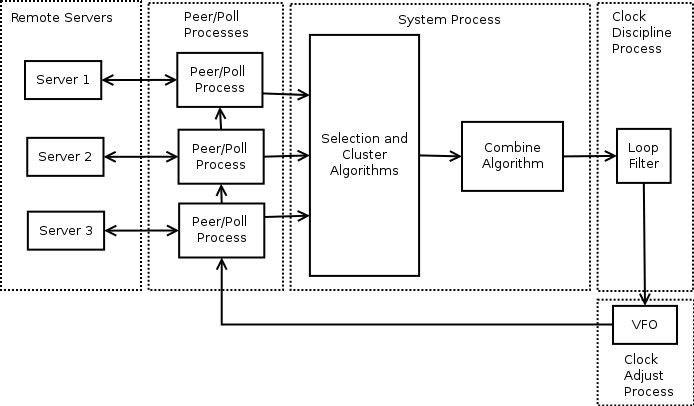
\includegraphics[scale=0.5]{image/ntp_implementation}
    \caption {Implementação dos processos executados por um nó da rede.}
    \label{fig:modelo}
\end{figure} 

\FloatBarrier

Cada componente é, portanto, responsável por uma funcionalidade específica
oferecida pelo NTP. Temos, assim:

\begin {enumerate}[i.]
  \item \textit{Remote servers}: servidores que fornecem sincronização aos nós
  da rede. Tais servidores podem pertencer à mesma rede às quais os clientes
  estão inseridos ou podem ser disponibilizados via Internet por organismos
  responsáveis por gerenciar e garantir que os relógios apresentem tempos
  consistentes. 
  
  A fim de diferenciar os diversos servidores utilizados em relação ao seu grau
  de importância e confiabilidade, o protocolo NTP atribui um nível a cada
  \textit{server}, chamado de \textit{stratum}. Tal atributo vale 1 para
  servidores primários, 2 para servidores secundários e assim sucessivamente. À
  medida que o valor de \textit{stratum} aumenta, a precisão diminui,
  dependendo do estado da rede. O valor máximo deste atributo é 15 e, portanto,
  são permitidos até 15 níveis hierárquicos. O valor 0 é reservado pelo
  protocolo para mensagens de controle e transmissão de estado entre nós. Tais
  mensagens são chamadas de pacotes \textit{Kiss-o'-Death}.
  
%   Caso \textit{stratum} de determinado servidor apresente o valor
%   16, isso significa que o cliente que está tentando obter sincronização está
%   dessincronizado com tal servidor.
  
  \item \textit{Peer/poll processes}: quando um pacote transmitido por um
  servidor chega em um nó, o \textit{peer process} é chamado. Tal processo então
  verifica se o pacote é consistente (\textit{On-Wire protocol}, proteção
  contra perdas e duplicatas) e calcula algumas estatísticas usadas pelos demais
  processos. Tais estatíticas consistem em:
  		
  		\begin{itemize}
  		  \renewcommand\labelitemi{--}
  		  \item \textit{offset} (\(\theta\)): deslocamento de tempo do
  		  relógio do servidor em relação ao relógio do sistema;
  		  \item \textit{delay} (\(\delta\)): tempo que o pacote necessita para
  		  percorrer toda a rede entre cliente e servidor;
  		  \item \textit{dispersion} (\( \epsilon \)): erro máximo inerente à medida
  		  do relógio do sistema;
  		  \item \textit {jitter} (\( \psi \)): raiz do valor quadrático médio dos
  		  \textit{offsets} mais recentes.
  		\end{itemize}
  		
	O \textit{poll process} é responsável, por sua vez, por enviar pacotes aos
	servidores a cada intervalo de \(2^\tau\) segundos. \(\tau\) varia de 4 a 17,
	resultando, assim, em intervalos de 16 segundos a 36 horas. O valor de \(\tau\)
	pode variar durante a execução, sendo modificado pelo algoritmo regulador do
	relógio, que será discutido posteriormente. 
	
	\item \textit{System process}: inclui algoritmos de seleção, clusterização e
	combinação que utilizam as diversas estatísticas obtidas de cada servidor para
	determinar os candidatos mais precisos e confiáveis à sincronização do relógio
	do sistema. As funções de cada algoritmo são, respectivamente:
		
		\begin{itemize}
  		  \renewcommand\labelitemi{--}
  		  \item determinar bons candidatos, isto é, determinar quais servidores
  		  possuem informações de sincronismo efetivamente importantes;
  		  \item determinar os melhores candidatos dentro do conjunto de servidores
  		  julgados importantes no passo anterior;
  		  \item computar estatísticas baseadas nos dados recolhidos dos servidores
  		  presentes no subconjunto escolhido pelo algoritmo de clusterição.
  		\end{itemize}
  	
  	\item \textit{Clock discipline process}: responsável por controlar o tempo e
  	frequência do relógio do sistema;
  	
  	\item \textit{Clock-adjust process}: roda a cada segundo para comunicar aos
  	demais processos os resultados das correções realizadas no relógio do
  	sistema.
  	
\end{enumerate}

\subsection {Exemplo}

A rede representada pela figura \ref{fig:redeNTP} foi proposta a fim de testar o
funcionamento do protocolo NTP. As setas determinam as relações entre os nós e
as direções representam quais nós fornecem e/ou recebem sincronização. Todos os
computadores pertencem à mesma rede, isto é, assume-se que há um \textit{router}
ligando esses nós e responsável pela comunicação com a Internet.

\FloatBarrier

\begin{figure}[h]
    
    \centering
    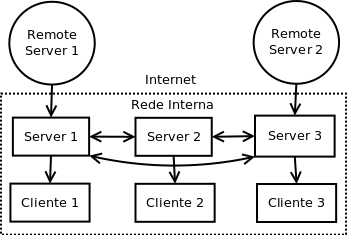
\includegraphics[scale=0.7]{image/rede_ntp_teste}
    \caption {Topologia da rede de teste.}
    \label{fig:redeNTP} 
\end{figure} 

\FloatBarrier

Têm-se, portanto, conforme a subseção anterior:

\begin{itemize}
  \renewcommand\labelitemi{--}
  \item associações cliente/servidor entre \textit{remote servers} e
  \textit{servers}, e entre \textit{servers} e \textit{clients};
  \item associações simétricas ativas entre \textit{servers}.
\end{itemize}

A fim de eliminar a necessidade de implementar essa rede fisicamente,
utilizou-se o \textit{software virtualbox}. Cada máquina presente na figura, com
exceção dos \textit{remote servers}, foi substituída por uma máquina virtual,
cujo sistema operacional é o \textit{Linux Debian 8.2.0 i386}. A escolha deste
sistema foi baseada nas características previstas para as máquinas que comporão
a infraestrutura do Sirius. Além disso, como pretende-se isolar completamente a
rede, isto é, eliminar qualquer comunicação com a Internet, os \textit{remote
servers} serão substituídos pelos respectivos servidores. Dessa maneira, tais
servidores utilizarão seus próprios relógios como fonte primária de sincronismo.

\vspace{12pt}

Foi adotado que a rede teria endereço \texttt{10.0.0.0/24}, os servidores
possuiriam endereços do tipo \texttt{10.0.0.10x}, sendo \textit{x} o dígito que
caracteriza o servidor (1, 2 ou 3), e \texttt{10.0.0.0y1} para os clientes,
sendo \textit{y} o equivalente de \textit{x}. 


\vspace{12pt}

Após a configuração de rede das respectivas máquinas virtuais, a instalação do
NTP pode prosseguir. Inicialmente, é necessário fazer a instalação do pacote
\texttt{ntp} através do comando

\begin{lstlisting}[language=bash, style=nonumbers]
$ sudo apt-get install ntp
\end{lstlisting}

Estão incluídos neste pacote, os programas \texttt{ntpd}, \texttt{ntpq}
e \texttt{ntpqc}. \texttt{ntpd}, ou \textit{NTP Daemon}, roda continuamente no
sistema e é responsável pela troca de mensagens com os diversos servidores
ou clientes, de acordo com as configurações, enquanto que \texttt{ntpq}
e \texttt{ntpqc} (o \textit{q} refere-se a \textit{query}) são utilizados para
verificar o estado das variáveis e alterar configurações do \textit{daemon}. 

\vspace{12pt}

Quando é iniciado, o \textit{daemon} retira as suas configurações do arquivo
\texttt{/etc/ntp.conf}. Cada nó da rede deve, portanto,
configurar esse arquivo de acordo com as funções que desempenha.

\vspace{12pt}

A configuração dos clientes é simples: basta adicionarmos a linha

\begin{lstlisting}[language=bash, style=nonumbers]
server 10.0.0.10y iburst
\end{lstlisting}

ao arquivo de configurações. A opção \texttt{iburst} é uma otimização fornecida
pelo protocolo que agiliza a sincronização inicial. Essa opção faz com que o
intervalo de envio de pacotes seja reduzido e a quantidade de pacotes
enviados seja aumentada caso o servidor não esteja acessível. 

\vspace{12pt}

Para o \textit{server 2}, é necessário adicionarmos as duas linhas seguintes.

\begin{lstlisting}[language=bash, style=nonumbers]
peer 10.0.0.101
peer 10.0.0.103
\end{lstlisting}

Essas duas linhas criam associações simétricas ativas entre o \textit{server 2}
e os outros servidores. Dessa maneira, eles poderão trocar informações de
sincronização entre si.

\vspace{12pt}

Para os servidores 1 e 3, além das duas linhas contendo a opção \texttt{peer}, é
necessário também adicionar as duas linhas abaixo:

\begin{lstlisting}[language=bash, style=nonumbers]
server 127.127.0.0
fudge 127.127.0.0 stratum 1
\end{lstlisting}

A primeira opção configura o relógio local do sistema como uma fonte de
sincronização, enquanto que a segunda aumenta a sua hierarquia. Se o
atributo \texttt{stratum} vale 1, logo a prioridade do respectivo servidor
torna-se máxima.

\vspace{12pt}

Para iniciar o \textit{daemon}, basta executar o comando abaixo em cada máquina.

\begin{lstlisting}[language=bash, style=nonumbers]
$ sudo /etc/init.d/ntp restart
\end{lstlisting}

Os sistemas levam alguns minutos para se sincronizarem. Para verificar o estado
das conexões e da sincronização, utiliza-se o programa \texttt{ntpq} através do
comando 

\begin{lstlisting}[language=bash, style=nonumbers]
$ ntpq -p
\end{lstlisting}

A opção \texttt{-p} lista todos os nós utilizados para sincronização do relógio
local. Para o \textit{Server 1}, espera-se uma saída parecida com a figura
\ref{fig:sv1} (não há garantias que seja idêntica, visto que os algoritmos que
determinam as fontes que serão utilizadas para sincronização são baseados em
fatores que podem variar dependendo do estado da rede). 

\FloatBarrier

\begin{figure}[h]
    
    \centering
    %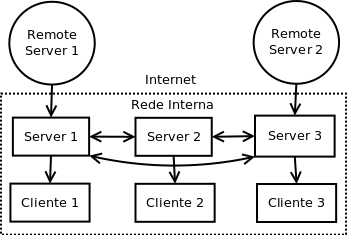
\includegraphics[scale=0.7]{image/rede_ntp_teste}
    \caption {Resultado do comando \texttt{ntpq -p} no \textit{Server 1}.}
    \label{fig:sv1} 
\end{figure} 

\FloatBarrier
\subsection {Aplicação ao projeto \textit{Sirius}} 

\section {Sincronização via \textit{Ethernet} com a \textit{BeagleBone Black}}

\subsection {Introdução}

A sincronização dos diversos componentes presentes no sistema de controle de um
acelerador de partículas é um fator fundamental para seu bom funcionamento. Os
sistemas que necessitam de sincronismo, como as fontes de corrente para os imãs,
controladores de feixe e de injeção, devem exercer as suas
respectivas funções em momentos especificados por pulsos de sincronismo, que
podem ser enviados, por exemplo, por geradores de sinais espalhados pela
infraestrutura local. A precisão com que estes equipamentos recebem tais pulsos
depende de diversas variáveis, como o tipo de canal de comunicação
utilizado no envio do pulso e a interface de entrada de dados que eles possuem.
A precisão pode ser obtida através da medição do \textit{jitter}, ou
desvio-padrão, do \textit{delay} calculado entre o envio do pulso e a sua
recepção no equipamento.
O \textit{Sirius}, por exemplo, possui especificações para diversos sistemas de
sincronismo, que variam de acordo com a necessidade de precisão dos equipamentos
e das funções desempenhadas por eles. Para casos mais graves, como o da bomba de
elétrons do acelerador linear (\textit{LINAC}), os \textit{jitters} não podem
ultrapassar os \textit{50ps} e soluções especiais devem ser exploradas, como a
implementação de uma rede \textit{WhiteRabbit}, que está sendo
desenvolvida e estudada por outros laboratórios no mundo todo.

\vspace{12pt}

Um sistema de sincronismo para as fontes de corrente já
foi implementado pelo grupo de controle, utilizando as unidades
\textit{Programmable Realtime Unit}, ou simplesmente \textit{PRU}, presentes na
\textit{BeagleBone}. Tais unidades apresentam \textit{clock} de 200MHz,
núcleos de memória própria e compartilhada, e módulos dedicados, como o
\textit{Enhanced GPIO}, que favorecem a implementação de aplicações
\textit{realtime}, em que a precisão é uma necessidade importante. Soluções
implementadas para a \textit{PRU} não estão sujeitas a fatores que degradam a
precisão como o compartilhamento de \textit{CPU} com outros
processos e preeempção. Aplicações que rodam sobre \textit{Linux} embarcado e
que, portanto, compartilham recursos com outros processos, apresentam,
geralmente, desempenho inferior. O sistema desenvolvido anteriormente pelo grupo
utiliza a \textit{PRU} para a recepção do sinal de sincronismo e ativa, posteriormente, seus nós
escravos, conforme figura \ref{fig:pru_sincronismo} abaixo. Esse sistema obteve
um \textit{jitter} da ordem de 18ns \cite{pat}, representando, assim, um valor
próximo do ótimo, uma vez que os ciclos de processamento de cada um dos componentes estão
próximos de 5ns.

\begin{figure}[h]

\centering
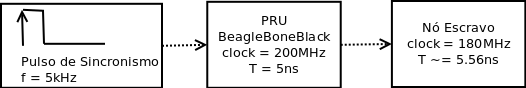
\includegraphics[scale=0.65]{image/pru_bbb_sincronismo}
\caption {Esquema de sincronismo realizado pelo grupo de controle.}
\label{fig:pru_sincronismo}
\end{figure}

\vspace{12pt}

Nesta seção, será apresentada a alternativa descrita na figura
\ref{fig:pru_sincronismo_ethernet}, que utiliza o protocolo \textit{Ethernet} e
equipamentos padrões na implementação deste tipo de rede, como
\textit{switches}, para o envio dos \textit{triggers} de sincronismo, e a sua
respectiva \textit{performance}. Duas implementações deste modelo serão
discutidas: uma em que tanto \textit{BB1} quanto \textit{BB2} executam
programas no \textit{kernel space}, chamados de \textit{kernel modules}, e a
outra, em que ambas utilizam seus módulos PRUs.

\vspace{12pt}

\begin{figure}[h]

\centering
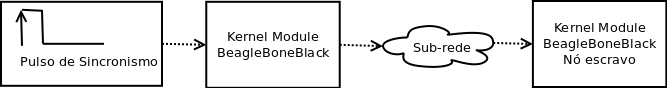
\includegraphics[scale=0.65]{image/pru_bbb_sincronismo_ethernet}
\caption {Sistema de sincronismo proposto.}
\label{fig:pru_sincronismo_ethernet}
\end{figure}

É importante observar que o modelo acima não pretende substituir a solução
implementada anteriormente pelo grupo \cite{pat} e que está atualmente em uso,
mas sim de contribuir para o aprendizado obtido durante o estágio.

\subsection {Implementação de \textit{Kernel Modules}}

Esta subseção é dedicada à primeira implementação do sistema de sincronismo
proposto.

\subsubsection{\textit{Loadable Kernel Modules}}

% A principal diferença entre os dois sistemas apresentados na subseção anterior é
% que, no segundo, não utilizamos a unidade \textit{PRU} da \textit{BeagleBone
% Black}. 
Nesta seção, propomos desenvolver módulos do
\textit{kernel} do \textit{Linux}, chamados de \textit{Loadable Kernel Modules} (\textit{LKM}).
Tais módulos são mecanismos que permitem a adição ou remoção de código do \textit{Linux kernel}
em tempo de execução e, por esta razão, são ideais para a implementação de
\textit{device drivers} \cite{derek}, cujo propósito principal é realizar a
comunicação com o \textit{hardware} disponível.  

\vspace{12pt}

Sendo essencialmente parte do \textit{kernel}, os \textit{LKMs} são executados
no \textit{kernel space} e, por isso, possuem endereços de memória e
\textit{APIs} próprios, que são, por sua vez, separados daqueles
disponíveis no \textit{user space}. Este último representa o \textit{space} em
que, na maioria das vezes, escrevemos e executamos as aplicações em C. A figura
\ref{fig:derek_kernel_user} resume as interações entre os dois espaços: o
\textit{user space} comunica-se com \textit{kernel space} através de
\textit{system calls}, que, por sua vez, acessa o \textit{hardware} através de
\textit{drivers} específicos. O \textit{kernel space} possibilita o tratamento
de interrupções, que serão utilizadas neste exemplo, ao contrário do
\textit{user space}.

\begin{figure}[h]

\centering
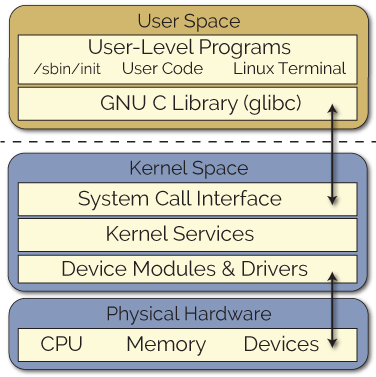
\includegraphics[scale=0.45]{image/userspace-kernelspace}
\caption {Comunicação entre \textit{kernel} e \textit{user spaces}. Extraída de
\cite{derek}.}
\label{fig:derek_kernel_user}
\end{figure}

\subsubsection{Descrição das características do projeto}

Neste projeto, utilizou-se duas \textit{BeagleBones Black}, denominadas
\textit{BB1} e \textit{BB2}, conforme figura \ref{fig:pru_sincronismo_ethernet}.
De maneira geral, foram desenvolvidas duas aplicações, uma para a \textit{BB1},
cujas funções são receber o \textit{trigger} de sincronismo e preparar o pacote
\textit{UDP} para envio, e a outra, para a \textit{BB2}, responsável pela
recepção do respectivo pacote e tratamento.
A aplicação que recebe o \textit{trigger} mantém um contador interno e o
transmite em intervalos definidos de tempo, para que o nó escravo possa também
manter um contador de mesmo tipo. Dessa forma, o nó escravo pode determinar se
um pacote foi perdido durante a transmissão e corrigir seu contador.

\vspace{12pt}

Em termos de programação, as aplicações apresentam as seguintes características:

\begin{itemize} \renewcommand\labelitemi{--}
  \item \textit{Kernel Module} em \textit{BB1}: um \textit{timer} gera
  interrupções a cada 1ms. Na rotina de tratamento desta interrupção, um
  registro contendo os dados a serem enviados via \textit{Ethernet} é
  adicionado em um \textit{buffer} circular. Uma outra \textit{thread}
  é responsável por retirar estes elementos do \textit{buffer}, prepapar os
  pacotes \textit{UDP} e enviá-los.

  \item \textit{Kernel Module} em \textit{BB2}: uma \textit{thread} é
  instanciada e espera pacotes \textit{UDP}. Quando recebe, atualiza seu
  contador e seus pinos de saída.
\end{itemize}

Por questões de simplicidade, o módulo \textit{PWM} da placa que envia os
pacotes \textit{UDP} (\textit{BB1}) será utilizado como gerador dos
\textit{triggers} de sincronismo. 

% \subsubsection {Configuração do \textit{PWM} com o \textit{Device Tree
% Overlays}}
% 
% Os mecanismos de \textit{Cape Manager} e \textit{Device Tree Overlays} permitem
% a modificação do sistema, como, por exemplo, configuração da função dos pinos,
% ativação e carregamento de módulos em tempo de execução a partir de programas
% sendo executados no \textit{user space}.
% 
% \vspace{12pt}
% 
% 
% Sendo assim, a fim de modificarmos o pino \texttt{P9\_22} (\textit{header P9},
% pino 22) para que atue como uma saída do módulo \textit{PWM}, é necessário
% escrevermos um arquivo de extensão \texttt{.dts} (\textit{device tree source}),
% contendo as especificações que desejamos adotar. Um arquivo deste tipo é
% disponível em \url{http://tinyurl.com/ntkl2w7} e contem todas as possíveis
% configurações de todos os pinos da \textit{BeagleBone Black}. Como vamos
% utilizar somente as linhas referentes ao \texttt{P9\_22}, podemos copiá-las para
% um arquivo separado e adotá-lo em seguida. Após obtermos tal arquivo, é
% necessário compilá-lo a partir do comando \texttt{dtc} e incluir o resultado no
% diretório \texttt{/lib/firmware/}.
% 
% \vspace{12pt}
% 
% Para carregar o \textit{overlay}, configuramos duas variáveis de ambiente:
% 
% \begin{lstlisting}[keywordstyle=\ttfamily, style=nonumbers]
% $ export SLOTS=/sys/devices/bone_capemgr.9/slots
% $ export PINS=/sys/kernel/debug/pinctrl/44e10800.pinmux/pins
% \end{lstlisting}
% 
% \vspace{12pt}
% 
% Executamos, então, os comandos abaixo, em que \texttt{pwm\_P9\_22} referencia o
% arquivo gerado após compilação. \texttt{duty\_ns} e \texttt{period\_ns}
% são utilizados, respectivamente, para configurar o intervalo de tempo em que a
% onda permanecerá em nível lógico alto e o seu período total. Para as próximas
% seções, vamos adotá-los como, respectivamente, 2\textit{ms} e 70\textit{ms}. Um
% \textit{script bash}, que pode ser encontrado no repositório do grupo, foi
% escrito e automatiza o processo abaixo.
% 
% \begin{lstlisting}[keywordstyle=\ttfamily, style=nonumbers]
% $ echo pwm_P9_22 > $SLOTS
% $ echo pwm > /sys/devices/ocp.3/P9_22_pinmux.12/state
% $ cd /sys/class/pwm/
% $ echo 0 > export 
% $ cd pwm0/
% $ echo 2000000 > duty_ns
% $ echo 70000000 > period_ns
% \end{lstlisting}

\subsubsection{Implementação do \textit{Kernel Module} de \texttt{BB1}}
\label{sec:bb1}

O \textit{module} desenvolvido para a placa \texttt{BB1} instancia duas
\textit{threads}: uma para inicialização dos componentes e a outra para
processamento e envio de pacotes \textit{UDP}. No \textit{kernel space}, cada
\textit{thread} é definida por uma estrutura do tipo \texttt{struct
task\_struct}, especificada na biblioteca \texttt{linux/kthread.h}, que provê também as funções
\texttt{kthread\_create} e \texttt{wake\_up\_process}. A primeira é reponsável
por alocar os recursos necessários à execução de uma \textit{thread} e a
segunda, por permitir a sua execução. É possível alterar a prioridade e a
\textit{policy} de uma \textit{thread} através da função
\texttt{sched\_setscheduler}, disponível em \texttt{linux/sched.h}. Esses dois
parâmetros são usados pelo \textit{Linux scheduler} para decidir qual dos
processos interrompidos deterá o processador após a interrupção ou bloqueio do
processo em curso de execução. O \textit{Linux} fornece duas políticas de
\textit{real-time}, \texttt{SCHED\_FIFO} e \texttt{SCHED\_RR}, que possuem
prioridade superior à politíca comum, \texttt{SCHED\_NORMAL}. Processos cujas
\textit{scheduler classes} são do tipo \textit{real-time} sempre são escolhidos
antes daqueles de política comum. É necessário observar que,  no \textit{kernel}
padrão do \textit{Linux},  estas classes não são capazes de garantir um
comportamento dito \textit{hard real-time} \cite{linuxlove}, isto é, que
asseguram o cumprimento de qualquer requisito dentro de um certo limite. As
\textit{real-time scheduling policies} fornecem, portanto, um comportamento de
\textit{soft real-time}, ou seja, o \textit{kernel} faz o máximo possível para
atender às requisições, mas não pode prometer sempre cumpri-las. Dada tal
limitação, um \textit{patch}, chamado \path{RT_PREEMPT} e disponível em
\cite{rt}, foi desenvolvido para garantir características de \textit{hard real-time}. Quando
uma tarefa do tipo \texttt{SCHED\_FIFO} assume a \textit{CPU}, ela continua a
ser executada até que ela seja bloqueada ou que ela conceda explicitamente o
processador a outro processo, podendo rodar indefinidamente caso nenhuma dessas
condições seja atendida. Somente uma tarefa \texttt{SCHED\_FIFO} ou
\texttt{SCHED\_RR} de maior prioridade pode interromper sua execução. Para as
tarefas do tipo \texttt{SCHED\_RR}, o princípio é o mesmo, porém elas são
submetidas a um intervalo de execução, sendo que, ao fim deste intervalo, tais
tarefas perdem os recursos de processamento e entram na fila circular de espera.
Em outras palavras, a política \texttt{SCHED\_RR} é semelhante à
\texttt{SCHED\_FIFO}, exceto no tempo que é permitido ao uso de \textit{CPU}. No
nosso caso, ambas as \textit{threads} terão políticas de \texttt{SCHED\_FIFO},
mas aquela que é interrompida pelo \textit{timer} e
\textit{GPIOs} possuirá maior prioridade. Em adição, a segunda \textit{thread}
(aquela responsável pelo envio de pacotes) desiste da \textit{CPU} quando o
\textit{buffer} circular está vazio e só é \textit{acordada} quando uma
interrupção de tempo ocorrer (o \textit{buffer} volta a ser preenchido na função de
tratamento desta interrupção). Os fluxogramas da figura \ref{fig:threads_bb1}
resumem o funcionamento destas \textit{threads}.

\vspace{12pt}

A figura \ref{fig:thread_int} especifica o fluxograma da \textit{thread\_int}
que preenche o \textit{buffer} circular a cada interrupção do relógio e sinaliza
para a \textit{thread\_proc} que ele não está mais vazio. A figura
\ref{fig:thread_proc} evidencia que um pacote é enviado somente se o
\textit{buffer} não estiver vazio. Caso contrário, a \textit{thread\_proc}
se bloqueia esperando uma interrupção do relógio. As funções \texttt{wake\_up} e
\texttt{wait\_event} estão disponíveis na biblioteca \texttt{linux/wait.h}. A
segunda deve receber como parâmetro uma fila, que representa a estrutura de
dados onde serão colocados os processos que esperam pelo evento. Essa fila é do
tipo \texttt{wake\_queue\_head\_t} e pode ser criada estaticamente, via
a \textit{macro} \texttt{DECLARE\_WAITQUEUE()}, ou dinamicamente, via a função
\texttt{init\_waitqueue\_head()}.

	\begin{figure}[h!]
	
	\centering
	
		\begin{subfigure}{.33\textwidth}
		  \centering
		  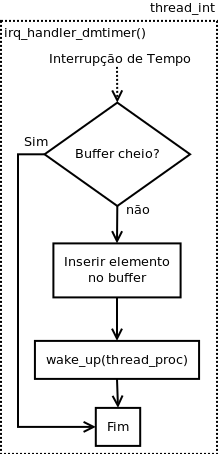
\includegraphics[scale=0.55]{image/thread_int}
		  \caption{\centering Fluxograma da \textit{thread} que é interrompida pelo
		  \textit{timer} de \texttt{BB1}.}
		  \label{fig:thread_int}
		  
		\end{subfigure}%
		\begin{subfigure}{.33\textwidth}
		  \centering
		  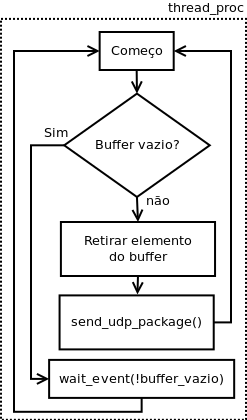
\includegraphics[scale=0.55]{image/thread_proc}
		  \caption{\centering Fluxograma da \textit{thread} que envia pacotes à
		  rede de \texttt{BB1}.}
		  \label{fig:thread_proc} 
		\end{subfigure}%
		\begin{subfigure}{.33\textwidth}
			\centering
			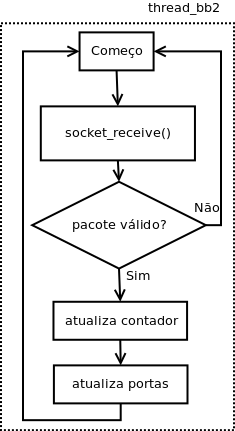
\includegraphics[scale=0.55]{image/thread_bb2}
			\caption {\centering Fluxograma da \textit{thread} do \textit{kernel module}
			em
			\texttt{BB2}.}
			\label{fig:thread_bb2}
		\end{subfigure}%
		\caption{Fluxogramas das \textit{threads} que compõem \texttt{BB1}
		e \texttt{BB2}.}
		\label{fig:threads_bb1}
		\end{figure} 

\vspace{12pt}

Os processadores da família \textit{Sitara AM335x} da \textit{Texas Instruments}
possuem um módulo, chamado de \textit{DMTimer}, composto por 7 \textit{timers}
configuráveis. Cada um dos \textit{timers} contém um contador de 32
\textit{bits} crescente com capacidade de \textit{auto reload} e geração de
interrupção ao atingir seu valor máximo (\texttt{0xFFFFFFFF}), isto é, em caso
de \textit{overflow}. Além disso, é possível configurar um divisor de frêquencia
(\textit{prescaler}) e escolher o sinal de \textit{clock} que será usado pelo
componente. No \textit{kernel space}, a biblioteca \texttt{plat/dmtimer.h}
fornece as principais operações para configuração do módulo. 

\vspace{12pt}

A função \texttt{omap\_dm\_timer\_request()} retorna uma estrutura do tipo
\texttt{struct omap\_dm\_timer} que representa um dos \textit{timers}
disponíveis no módulo. Há mais algumas variantes desta chamada, porém a
principal é a \texttt{omap\_dm\_timer\_request\_specific(int timer\_id)}, que
recebe como parâmetro o \textit{id} do \textit{dmtimer} desejado. É necessário
notar, porém, que talvez seja necessário a configuração de um \textit{overlay}
para a configuração dos pinos utilizados pelo respectivo \textit{timer}. Em
seguida, executamos a chamada \path{omap_dm_timer_set_source}, que
configura o sinal de \textit{clock} de entrada. Utilizamos o \textit{clock} de
32kHz, portanto passamos a constante \texttt{OMAP\_TIMER\_SRC\_32\_KHZ} como
parâmetro à função. \texttt{omap\_dm\_timer\_set\_prescaler} permite definir o
valor do divisor de frequência e \path{omap_dm_timer_set_load_start}, o
valor que será carregado no contador quando um \textit{overflow} ocorrer. Tais
definições dependem do intervalo desejado entre interrupções e são dadas pela
equação \ref{eq:timer}, em que \textit{TDLR} é o valor a ser carregado no
contador, \textit{PTV}, o \textit{prescaler} e \(f_{clock}=32kHz\).

\begin{equation} 
t = (\text{0xFFFFFFFF} - TDLR + 1)*\frac{1}{f_{clock}}*2^{PTV+1}
\label{eq:timer}
\end{equation}

No nosso caso, desejamos interrupções a cada \(t=1ms\) com \(PTV=1\). A
aplicação direta da equação \ref{eq:timer} resulta em \textit{TDLR} =
0xFFFFFFF7.

\vspace{12pt}

O último passo é ativar a interrupção em caso de \textit{overflow} e associar a
ela uma função de tratamento. Para configurá-la, utilizamos três funções:

\begin{itemize} \renewcommand\labelitemi{--}
  \item \texttt{omap\_dm\_timer\_get\_irq()}: retorna o \textit{id} da
  interrupção associada ao \textit{timer} passado como parâmetro;

  \item \texttt{omap\_dm\_timer\_set\_int\_enable()}: habilita interrupção no
  módulo. Recebe como parâmetro uma constante que define o evento que deve ser
  associado à interrupção. No nosso caso, como queremos que uma interrupção seja
  lançada após \textit{overflow} do contador, passamos o valor
  \path{OMAP_TIMER_INT_OVERFLOW};

  \item \texttt{request\_irq()}, da biblioteca \texttt{linux/interrupt.h}:
  recebe como parâmetro o \textit{id} da interrupção, a sua função tratadora e
  o tipo de função. Este último é uma constante definida na biblioteca e vale
  \path{IRQF_TIMER}. No nosso caso, criamos uma função chamada
  \path{dmtimer_irq_handler()} que retorna uma estrutura do tipo \texttt{irqreturn\_t}. Para comunicar ao sistema
  operacional que a interrupção foi corretamente tratada, tal função deve
  retornar \texttt{IRQ\_HANDLED}. Além desta constante, a função deve atualizar
  o registrador de \textit{status} do módulo realizando uma escrita. Isso é
  feito através da função \texttt{omap\_dm\_timer\_write\_status()}, com o
  parâmetro \path{OMAP_TIMER_INT_OVERFLOW}.
\end{itemize}
 
Enfim, iniciamos o \textit{timer} com a chamada de \path{omap_dm_timer_start()}.

\vspace{12pt}

A próxima etapa é a configuração dos pinos de entra e saída. A biblioteca
\texttt{linux/gpio.h} fornece as funções necessárias para definirmos a direção
(entrada ou saída) e o nível lógico a ser atribuído a um respectivo pino.
Utilizamos dois pinos de entrada e saída nesta aplicação:

\begin{itemize} \renewcommand\labelitemi{--}
  \item \texttt{GPIO\_48} (\texttt{P9\_15}): pino de entrada que recebe o
  \textit{trigger} de sincronismo. A cada borda de subida detectada, uma
  interrupção é lançada e algumas \textit{flags} responsáveis por armazenar a
  ocorrência do evento são atualizadas. Quando a \textit{thread\_proc} prepara o
  próximo pacote, ela consulta essas \textit{flags} e, caso estejam
  \textit{setadas}, adiciona ao respectivo pacote o \textit{trigger} recebido;

  \item \texttt{GPIO\_68} (\texttt{P8\_15}): pino de saída que tem seu valor
  alterado quando um \textit{trigger} de sincronismo foi detectado. Utilizado
  para testes da aplicação.
\end{itemize}

Para verificar se um pino pode ser utilizado, chamamos a função
\path{gpio_is_valid}, cujo parâmetro é o \textit{id} do respectivo pino. Se o
retorno for diferente de 0, o \textit{id} é valido e podemos continuar a
configurá-lo. Em seguida, executamos, em sequência,
\path{gpio_request()}, \path{ gpio_direction_output()} - para saída - ou
\path{gpio_direction_input()} - para entrada - e \path{gpio_export()}. Tais
funções são responsáveis por, respectivamente, reservar o pino, configurar sua
direção e exportá-lo, permitindo ou não que outras aplicações o utilizem. O pino
de entrada requer adicionalmente que uma interrupção seja relacionada a ele.
Para tal, repetimos o procedimento realizado para o \textit{timer}, isto é,
obtemos o \textit{id} da interrupção através de \path{gpio_to_irq()} e associamos
uma função tratadora com \path{request_irq()}. Entretanto, ao invés de enviarmos
o parâmetro \path{IRQF_TIMER} para esta última, passamos
\path{IRQF_TRIGGER_RISING}, que lançará as interrupções quando bordas de subida
forem detectadas. Em relação aos pinos de saída, utiliza-se 
\path{gpio_set_value()} para modificar o valor de tensão imposta na respectiva
saída, cujo \textit{id} é passado como parâmetro à função. Os recursos
utilizados por um pino de entrada ou saída são liberados a partir das chamadas
\path{gpio_unexport()} e \path{gpio_free()}.

\vspace{12pt}

Enfim, o último aspecto a ser discutido neste módulo é a implementação do envio
de pacotes \textit{UDP}. Três bibliotecas devem ser importadas a fim de realizar
essa comunicação: \path{linux/netdevice.h}, \path{linux/ip.h} e
\path{linux/in.h}. O primeiro passo é a criação do \textit{socket} de
comunicações, que é realizado pela chamada à função \path{sock_create()},
passando como parâmetros algumas constantes e a estrutura \texttt{struct socket}
que representa um \textit{socket} no \textit{kernel space}. As constantes
especificam o tipo do respectivo \textit{socket}, sendo que, para aplicações
\textit{UDP}, utilizamos \path{AF_INET}, \path{SOCK_DGRAM} e \path{IPPROTO_UDP},
que especificam, respectivamente, o formato dos endereços (endereços
\textit{Internet Protocol v4}), as camadas de transporte e rede dos pacotes a
serem enviados. Em seguida, definimos seu endereço e a porta a partir da função
\path{connect()}, que pode ser acessada através do atributo \path{ops} de
\texttt{struct socket}. Além do \textit{socket} criado, ela recebe como
parâmetro um ponteiro para uma variável do tipo \texttt{struct sockaddr}, que,
por sua vez, possui três atributos importantes: \path{sin_family},
\path{sin_addr.s_addr} e \path{sin_port}. Recebem, respectivamente,
\path{AF_INET}, \path{htonl(INADDR_SEND)} e \path{htons(CONNECT_PORT)}, em que
\path{htonl()} e \path{htons()} são funções pré-definidas que convertem valores
de \textit{host order} para \textit{network byte order} (\path{0xc0a80216} para
\path{192.168.2.22}, por exemplo), \path{INADDR_SEND} é o endereço para o qual
deseja-se enviar datagramas e \path{CONNECT_PORT} é a porta.
\path{connect()}, além de definir tais características, também ativa a conexão
no \textit{socket}. O envio de pacotes é realizado por \path{sock_sendmsg()},
que recebe dois parâmetros: as estruturas \texttt{struct socket} e
\texttt{struct msghdr}, que contém o conteúdo da mensagem. Enfim, para desalocar
o \textit{socket}, chama-se a funçao \path{sock_release()}.

% \vspace{12pt}
% 
% Por fim, a compilação do arquivo \path{.c} é realizada por meio de um
% \textit{Makefile}, cujo conteúdo é semelhante ao código abaixo, em que
% \path{timer_kernel_module} é o nome do arquivo do módulo e \texttt{\$(shell
% uname -r)} retorna a versão dos \textit{linux headers} instalados na
% \textit{Beagle}.
% 
% \begin{lstlisting}[keywordstyle=\ttfamily, style=nonumbers]
% obj-m+=timer_kernel_module.o 
%  
% all:
% 	make -C /lib/modules/$(shell uname -r)/build/ M=$(PWD) modules 
% clean:
% 	make -C /lib/modules/$(shell uname -r)/build/ M=$(PWD) clean
% \end{lstlisting}

% \vspace{12pt}
% 
% A adição do módulo compilado (arquivo \path{.ko}) é realizado através do comando
% \path{insmod} e a sua remoção, a partir de \path{rmmod}. O arquivo
% de \textit{log} pode ser utilizado para eventual \textit{debug}, sendo acessado
% a partir de \path{/var/log/kern.log}.

\subsubsection{Implementação do \textit{Kernel Module} de \texttt{BB2}}

Uma só \textit{thread} é instanciada no \textit{kernel module} de \texttt{BB2}.
Ela aguarda a recepção de pacotes \textit{UDP} e os processa. Ela é criada da
mesma forma descrita na subseção anterior e tem sua \textit{policy} modificada
para \path{SCHED_FIFO}, a fim de obter tratamento de \textit{real-time}. O
fluxograma da figura \ref{fig:thread_bb2} destaca a execução do módulo. Quando
um pacote é recebido, há uma verificação de sua integridade e, caso seja válido,
o contador e as portas de \textit{gpio} são atualizadas conforme conteúdo.
Observa-se que o processo de inicialização de tais portas segue o mesmo
princípio que o descrito em \textbf{Implementação do \textit{Kernel Module} de
\texttt{BB1}}. A criação do \textit{socket}, no entanto, é ligeiramente
diferente: ao invés da função \path{connect()}, utiliza-se \path{bind()}, que
atribui um endereço e porta ao respectivo \textit{socket}, passado como
parâmetro através de uma estrutura do tipo \texttt{struct sockaddr}, que é
inicializada com as funções \texttt{htonl} e \texttt{htons}, destacadas
anteriormente. A recepção dos pacotes é feita via \path{sock_recvmsg()}, que
bloqueia a \textit{thread} até que um datagrama seja detectado.
% 
% \vspace{12pt}
% 
% A compilação pode ser feito através de um \textit{Makefile} e a adição e remoção
% do módulo, via os comandos \path{insmod} e \path{rmmod}.


\subsection{Utilizando o módulo PRU}

Implementações alternativas para os \textit{kernel modules} de \textit{BB1} e
\textit{BB2} foram propostas usando o módulo PRU da \textit{BeagleBone Black}.
Para \textit{BB1}, a configuração do \textit{timer} e a verificação das
interrupções geradas por ele e pelo pulso de sincronismo são feitas pela PRU.
Quando um \textit{trigger} é recebido, um sinal é enviado para um programa
rodando no \textit{user space} da \textit{Beagle}, cujo propósito é, de fato,
enviar pacotes \textit{UDP} para \textit{BB2}. É importante observar que a
comunicação entre o processador e o módulo PRU é garantida via \textit{hardware}
e que uma API contendo funções de comunicação com a PRU também é fornecida pela
comunidade.

\vspace{12pt}

Um processo semelhante foi realizado para \textit{BB2}, isto é, substituiu-se o
\textit{kernel module} por um programa rodando na unidade de tempo real. Tal
programa verifica, através de \textit{polling} nos registradores do controlador
de rede, se um novo pacote foi recebido. Se isto ocorreu, então um sinal é
enviado a um outro programa no \textit{user space}, responsável por tratar tal
pacote. O tratamento de tal pacote não é realizado diretamente na PRU, visto que
seria necessária a implementação de toda a pilha \textit{UDP/IP}.

\subsection {Resultados}

Para avaliar os resultados, conectamos o \textit{PWM} ao canal 3 do osciloscópio
e configuramos o \textit{trigger} para detectar subidas de borda deste canal. O
módulo de \texttt{BB2} foi configurado para modificar o estado de um pino de
saída, ao qual conectamos ao canal 2, a fim de gerar um simples pulso quando um
pacote contendo um \textit{trigger} de sincronismo for recebido. Dessa forma,
podemos avaliar o \textit{delay} entre a criação do evento inicial e de sua
recepção no nó escravo, assim como o \textit{jitter} associado. Para tal,
utilizamos a ferramenta \textit{Histograma} disponibilizada no equipamento e a
configuramos para adquirir medidas relacionadas ao canal 2, isto é, pulsos
gerados pela \textit{Beagle} \texttt{BB2}. Modificamos a opção \textit{Tempo de
Persistência} do \textit{Display Forma de onda} para infinito, de forma a
garantir que a tela do osciloscópio mantenha os pulsos gerados em instantes
anteriores. Enfim, habilitamos o funcionamento do osciloscópio, obtendo o
resultado presente na figura \ref{fig:osciloscopio_thread} para a implementação
contendo os \textit{kernel modules} e na \ref{fig:pru_osciloscopio_thread} para
a implementação utilizando a PRU. Os desvios padrões, ou \textit{jitters},
obtidos são, respectivamente, 5.7\textit{ms} e 985.1\(\mu s\), muito distantes
daquele adquirido pelo sistema construído pelo grupo de controle, no qual
utilizou-se somente a \textit{PRU} e obteve-se um valor próximo de
18\textit{ns} \cite{pat}. Tal diferença é explicada, basicamente, por dois
fatores: o canal utilizado para envio da mensagem e o componente de processamento da
\textit{Beagle}. Nas nossas aplicações, utilizamos um \textit{switch HP V1810G},
que apresenta um comportamento \textit{não determinístico}, isto é, não é
possível prever com certeza o tempo necessário para que um pacote seja
entregue a um determinado \textit{host}. O segundo aspecto a ser considerado é
que aplicações rodando na \textit{PRU} não dividem recursos com outros
processos, ao contrário de aplicações que rodam em \textit{embedded linux}. Na
seção \ref{sec:bb1}, comentamos que, apesar do \textit{Linux} fornecer políticas
de preempção \textit{real-time}, o comportamento chamado de \textit{hard
real-time} não poderia ser alcançado pelo \textit{kernel}. Em oposição, as
unidades \textit{PRUs} da \textit{Beagle} foram desenvolvidas para este
propósito.

\begin{figure}[h]

\centering
	\begin{subfigure}[t]{0.5\textwidth}
		\centering
		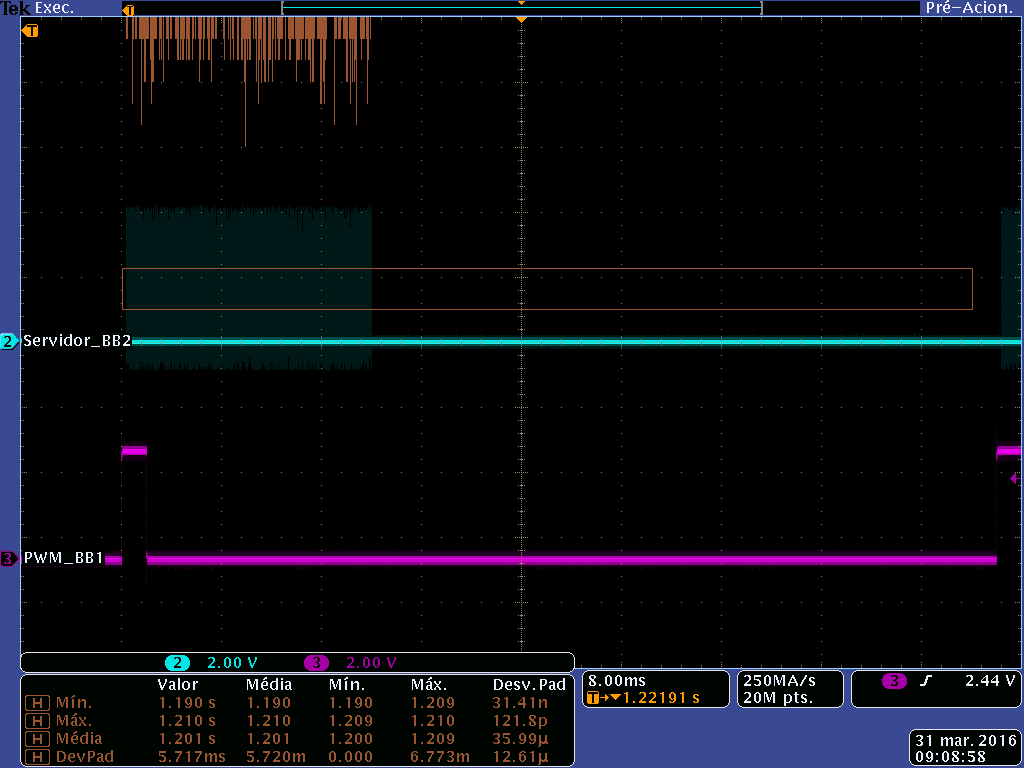
\includegraphics[width=0.95\textwidth]{image/tek_com_threads}
		\caption {\centering Captura de tela do osciloscópio para a implementação com
		\textit{kernel modules}.}
		\label{fig:osciloscopio_thread}
	\end{subfigure}%
	\begin{subfigure}[t]{0.5\textwidth}
		\centering
		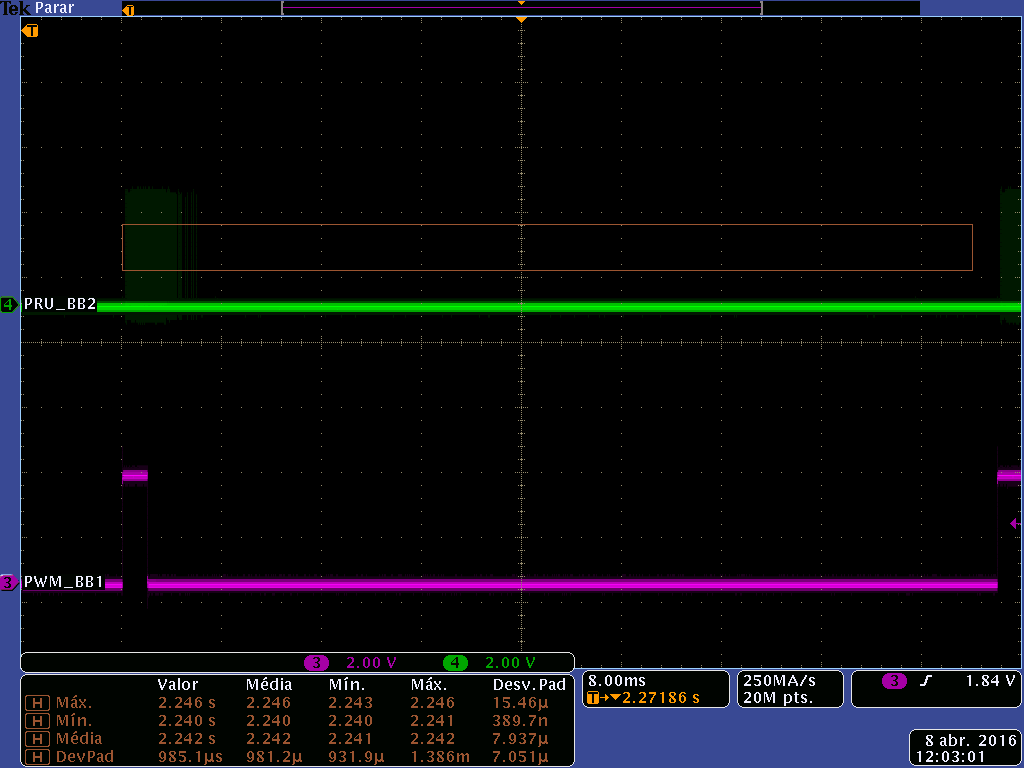
\includegraphics[width=0.95\textwidth]{image/tek_pru}
		\caption {\centering Captura de tela do osciloscópio para implementação com
		PRU.}
		\label{fig:pru_osciloscopio_thread}
	\end{subfigure}%
	
	\caption {Resultados encontrados para as duas implementações.}
\end{figure}

\subsection{Alternativas de solução}

Nesta subseção, serão introduzidas algumas alternativas que também utilizam
\textit{Ethernet} como meio de comunicação de \textit{triggers} de sincronismo.

\subsubsection{\textit{Industrial Ethernet}}

Alguns protocolos foram desenvolvidos a fim de alcançar exigências de
\textit{hard real-time} sobre redes \textit{Ethernet}. Um deles é o
\textit{EtherCAT} (\textit{Ethernet for Control Automation Technology}),
desenvolvido pela empresa alemã \textit{Beckhoff}, que utiliza as unidades de
processamento \textit{real-time} (\textit{PRUs}). Um dos incovenientes desta
aplicação em relação à \textit{BeagleBone Black} é que o seu processador,
\textit{Sitara AM3358}, não suporta este protocolo, sendo que os únicos da mesma
família que o suportam são \textit{AM3357} e \textit{AM3359}. A \textit{Texas
Instruments} fornece um \textit{kit} de desenvolvimento com o último, chamado de
\textit{AM3359 Industrial Communications Engine}, e uma biblioteca desenvolvida
para o uso deste protocolo, \textit{SYS/BIOS Industrial Software Development Kit
(SDK)}. Além do \textit{EtherCAT}, outras alternativas para comunicação
\textit{real-time} sobre \textit{Ethernet} e que são suportadas pelo processador
AM3358 são \textit{Ethernet/IP}, \textit{PROFINET RT/IRT} e \textit{PROFIBUS}.

\subsubsection{\textit{Time Sensitive Networking}}

\textit{Time Sensitive Networking (TSN)} é um conjunto de padrões IEEE802 que
extende as funcionalidades de uma rede \textit{Ethernet} e
implementa mecanismos de sincronização temporal e escalonamento capazes de
assegurar transmissões determinísticas sobre \textit{Ethernet}
padrão \cite{marcio}. É importante observar também que o \textit{TSN}
permanece compatível com a pilha TCP/IP.

\vspace{12pt}

Essa tecnologia ainda está em fase inicial de desenvolvimento, tendo sido
anunciada neste mesmo ano de 2016.




\section {Manutenção do PROSAC e Implementação de Aplicações Clientes}

\subsection{Introdução}

O \textit{PROSAC} é um \textit{firware} desenvolvido no grupo de controle, cujo
principal propósito é receber requisões da sala de controle e acionar a
respectiva placa do bastidor. Esse \textit{firware} apresenta, atualmente,
suporte a diversas placas que são usadas atualmente no \textit{UVX} para
controle de fontes e monitoramento de sensores. Exemplos de placas operadas pelo
\textit{PROSAC} são a \textit{LOCON} de 12 e 16 \textit{bits}, a
\textit{STATFNT} e a \textit{DIGINT}.

\vspace{12px}

Considerando a sua importância no contexto do sistema controle, dois clientes
foram implementados a fim de testar seu funcionamento: um em Java e outro,
utilizando o \textit{kit} de desenvolvimento \textit{STM32F7 Discovery}.

\subsection {Manutenação do \textit{PROSAC}}

O grupo de controle publicou na PCaPAC 2016 um artigo entitulado \textit{UVX
Control System: An Approach With BeagleBone Black} \cite{pcapac2016}, em que fui
um dos autores. Minha tarefa neste trabalho, em poucas palavras, foi ajustar a
política de escalonamento e a prioridade das \textit{threads} que compõem o
\textit{PROSAC}, de forma a obter o melhor desempenho possível nas tarefas
síncronas realizadas pelo programa. As tarefas ditas \textit{síncronas}
são aquelas que necessitam ser sincronizadas a partir de um pulso de sincronismo
externo. No \textit{PROSAC}, tais tarefas consistem nas operações de ciclagem e
rampa, isto é, a cada novo pulso recebido, o \textit{PROSAC} é encarregado de
transmitir um novo valor às placas que estiverem participando do processo.
Devido às mesmas limitações de processamento de tempo real discuitidas na seção
\ref{sec:bb1}, o número de pulsos perdidos na nova versão do \textit{PROSAC} era
elevado para as frequências superiores a 500Hz, que tornava o seu uso
proibitivo. Dessa forma, prôpus utilizarmos o \textit{scheduler} denominado de
\textit{Completely Fair Scheduler} e ajustar a prioridade das \textit{threads}
de forma a garantir um maior tempo de CPU à \textit{thread} responsável por
processar os pulsos. A tabela \ref{tab:prosac} a seguir ilustra a taxa de pulsos
perdidos para a configuração do \textit{PROSAC} com o \textit{Completely Fair
Scheduler} conectado a duas placas LOCON de \textit{12 bits}, ambas
participando da ciclagem. Conforme tabela, as taxas de pulsos perdidos são muito
inferiores aos pulsos totais recebidos, possibilitando, assim, seu uso no UVX.

\vspace{-12pt}

\begin{table}[h]

	\centering
	\caption{\label{tab:prosac} Resultados do \textit{PROSAC} com o
	\textit{Completely Fair Scheduler}.}
	\begin{tabular}{| c | c | c | c |}
		\hline
		\textbf{Frequência (Hz)} & \textbf{Pulsos perdidos} & \textbf{Total} &
		\textbf{Razão} \\ \hline 
		150 & 0 & 579.812  & 0 \\ \hline
		512 & 8 & 5.376.056 & 0.0001\% \\ \hline
		1000 & 18 & 6.050.225 & 0.0003\% \\ \hline
	\end{tabular}	    
\end{table}
 
 
\subsection {Manutenção do cliente \textit{PROSAC} escrito em \textit{Java}}

O cliente \textit{PROSAC} implementado em \textit{Java} foi desenvolvido em 2011
por Bruno Martins para testes iniciais do \textit{PROSAC}. Desta forma, casos mais
complexos, como placas desenvolvidas posteriormente ao cliente, produziam
exceções que interrompiam o programa. As seguintes modificações foram realizadas
a fim de corrigir tais problemas:

\begin {enumerate} [i.] 
  \item Função \texttt{processCommand} da classe \texttt{Client}: foi adicionado
  uma condição para verificar se a quantidade de \textit{bytes} recebidos do
  \textit{PROSAC} é a mesma que a esperada. Tal condição encontra-se no laço
  \texttt{for} do bloco \texttt{default} do \texttt{switch}.

  \item Modificação de forma que os \textit{status} das placas apareçam em uma
  janela distinta daquela onde o painel de comando está inserido. A classe
  \texttt{Boards} foi substituída pela \texttt{BoardsFrame}.
  
  \item Suporte às placas \textit{Statfnt}, \textit{Digint}, \textit{Rux} 12
  \textit{bits} bipolar e \textit{Mux} 16 \textit{bits}, e implementação das
  respectivas interfaces gráficas.

  \item Correção nas escalas dos gráficos para as placas monopolares de 12 e 16
  \textit{bits}.
  
  \item Para a operação de rampa, o \textit{PROSAC} necessita da ordem com que
  as placas aparecem no bastidor, não seus \textit{IDs}. Por exemplo, se duas
  placas estiverem presentes, cujos \textit{IDs} são 5 e 19, e quisermos
  executar uma rampa na 5, temos que enviar sua posição do bastidor, isto é 0.

\end{enumerate}

\subsection {Implementação para o \textit{kit} \textit{STM32F7 Discovery}}

O \textit{kit} \textit{STM32F7 Discovery} oferece diversos recursos
como interface \textit{Ethernet}, \textit{I2C}, \textit{UART} e tela
\textit{LCD Touch} capacitiva. Os principais passos na implementação desta
solução foram:

\begin{enumerate} [i.]
  \item Configuração de plugins para desenvolvimento na \textit{IDE Eclipse}.
  \item Configuração da interface \textit{OpenOCD}, responsável pela comunicação
  entre placa e computador.
  \item Implementação de um projeto na aplicação \textit{STMCubeMX} para
  inicialização dos pinos dos módulos que serão utilizados no projeto.
  \item Adição dos \textit{middlewares} \textit{FreeRTOS} e \textit{LwIP} ao
  projeto.
  \item Correção do \path{stm32f7_hal_conf.h} com a definição dos
  registradores corretos do módulo \textit{PHY}.
  \item Criação de uma interface gráfica, capaz de reconhecer
  eventos de \textit{touch}.
\end{enumerate}

A lógica utilizada nesta aplicação foi adaptada do cliente \textit{Java} e,
portanto, apresenta os mesmos comportamentos. Duas \textit{threads} são criadas,
sendo que uma envia requisições de leitura de dados a todo momento ao
\textit{PROSAC} e a outra, comandos requisitados pelo usuário, como ciclagem e
rampa.


% \section{Servidores de variáveis EPICS}
\label{sec:pcaspy}

\subsection{Introdução}

\textit{EPICS}, do inglês \textit{Experimental Physics and Industrial Control
System}, é um conjunto de ferramentas e aplicações que permitem monitorar e
controlar sistemas que possuem, além de milhares de variáveis, uma larga e
complexa rede ligando centenas de computadores e equipamentos. Tal sistema já é
utilizado em diversos outros síncrotons e laboratórios no mundo todo e o seu
desenvolvimento é realizado cooperativamente entre tais organizações. O
principal intuito é proporcionar aos operadores de sistemas de grande porte uma
visão global dos diversos módulos, facilitando, desta maneira, a identificação e
previsão de problemas, assim como a escolha da melhor ação corretora. Entre as
ferramentas oferecidas, destaca-se, por exemplo, arquivadores de variáveis,
monitores de alarmes e suporte para construção de \textit{interfaces} gráficas
específicas para determinadas aplicações, que serão discutidos nas próximas
seções deste documento.

\vspace{12pt}

Atualmente, no \textit{UVX}, o controle é realizado através de módulos
independentes, muitas vezes implementados em linguagens de programação
distintas, que fornecem soluções específicas para um determinado equipamento e
baixo grau de interação com outros programas. A identificação de problemas é,
portanto, dificultada e depende muito mais de experiências anteriores dos
operadores. Sendo assim, a implementação de \textit{EPICS} para o sistema
controle do \textit{Sirius} está sendo considerada fortemente. Além disso, o
acelerador linear de eléctrons, que está sendo atualmente desenvolvido por uma
empresa chinesa, a ser utilizado neste novo síncroton também oferecerá  uma
\textit{interface} de comunicação com total compatibilidade com aplicações
\textit{EPICS}.

\vspace{12pt}

De maneira simples, um sistema \textit{EPICS} é composto por diversos
servidores e clientes espalhados pela rede, capazes, respectivamente, de
publicar ou obter os estados dos diversos dispositivos pertencentes à estrutura.
Tais estados são chamados de variáveis, ou somente \texttt{PVs}, e podem
assumir vários tipos (binário, inteiro, \textit{float} \ldots), faixas de
operação e taxas de aquisição que dependem principalmente da maneira de como os
equipamentos proveêm tais dados. Cabe aos servidores (chamados também de
\textit{Input/Output Controllers} ou \textit{IOCs}), portanto, realizar as
operações de escrita ou leitura no \textit{mundo real} ou obter tais informações
de outros dispositivos, como osciloscópios e sensores, e publicá-las aos
clientes. A comuncicação entre clientes e servidores é realizado através do
protocolo de rede \textit{Channel Access}, implementado para redes que oferecem
grande largura de bandura, capaz de garantir o atendimento de especificações de
\textit{soft real-time} (consultar seção \ref{sec:bb1} para mais informações).

\vspace{12pt}

As próximas subseções serão dedicadas ao detalhamento de duas possíveis
implementação de servidores de variáveis. A primeira utiliza a biblioteca
\path{pcaspy} de \textit{Python}, enquanto que a outra, um módulo chamado
\path{StreamDevice}.

\subsection{Utilizando a biblioteca \texttt{PCASpy}}

O módulo \path{PCASpy} (\path{PCAS} do inglês \textit{Python Channel Access
Server}) fornece classes que realizam tanto a comunicação com um cliente
\textit{Channel Access} quanto com os dispositivos medidores. Esse módulo
oferece quatro classes, porém, em princípio, utiliza-se apenas duas, sendo elas
\path{SimpleServer} e \path{Driver}.

\vspace{12pt}

A classe \path{SimpleServer} abstrai os detalhes da comunicação entre servidor e
clientes e redireciona requisições de leitura e escrita para um objeto da classe
\path{Driver}, que por sua vez, se comunica com o dispositivo medidor. Um objeto
da classe \path{SimpleServer}, portanto, é a ponte entre os clientes e tais
equipamentos. Entre seus métodos, destaca-se:

\begin{itemize}
  \renewcommand\labelitemi{--}
  \item \texttt{createPV(\textit{prefix}, \textit{pvdb})}: registra e torna
  disponível as variáveis contidas no dicionário \texttt{\textit{pvdb}}. A
  documentação do módulo na \textit{Internet} contem os campos válidos para
  configuração de uma \texttt{\textit{PV}}.

  \item \texttt{process(\textit{time})}: o servidor processa requisições dos
  clientes a cada \texttt{\textit{time}} segundos.
\end{itemize}

A classe \texttt{Driver} deve ser redefinida a fim de refletir os detalhes de
comunicação e protocolo.  Para tal, através de mecanismos de herança,
redefine-se os métodos \texttt{\textit{read()}} e \texttt{\textit{write()}}, que
realizam, respectivamente, a leitura e escrita de variáveis. Além destas duas
funções, essa classe mantém um registro interno dos valores das variáveis. Para
modificá-lo, dois outros métodos são usados, sendo eles
\texttt{\textit{getParam()}} e \texttt{\textit{setParam()}}. Enfim, a função
\texttt{\textit{updatePV()}} é chamada para comunicar ao objeto
\path{SimpleServer} que uma \textit{PV} foi modificada.

\subsection{\textit{EPICS StreamDevice}}

O EPICS \textit{StreamDevice} oferece suporte para a comunicação com
dispositivos que podem ser controlados através do envio de \textit{strings},
isto é, cadeias de \textit{bytes}. Dessa forma, dispositivos que possuem
interface \textit{serial} de dados, como os padrões RS-232 e RS-485, podem se
comunicar com um \textit{StreamDevice} e fornecer os valores para as diversas
variáveis EPICS configuradas.

\vspace{12pt}

A configuração de um \textit{StreamDevice} é realizada a partir de arquivos
ditos do tipo \textit{protocolo}. Tais arquivos especificam os formatos e os
padrões que são entendidos pelo dispositivo e determinam, portanto, os
\textit{bytes} que devem ser enviados para cada tipo de operação. Muitas opções
de comandos e formatos são disponíveis nesta ferramenta, sendo que as principais
serão detalhadas nas próximas subseções. As variáveis que são disponibilizadas à
rede são, por sua vez, especificadas no arquivo \textit{database}, que é lido
durante a inicialização de um \textit{StreamDevice}. As operações de leitura e
escrita destas respectivas variáveis devem estar presentes em um dos arquivos de
\textit{protocolo}.

\vspace{12pt}

A comunicação das mensagens para o meio físico propriamente dita não é realizada
pelo \textit{StreamDevice}. Por padrão, tal ferramenta possui uma
\textit{interface} com um \textit{driver} de comunicação assíncrona chamado
\textit{asynDriver}, que deve ser instalado separadamente. De modo prático, o
módulo \textit{StreamDevice} é responsável por converter os \textit{bytes}
recebidos e enviados em variáveis EPICS, enquanto que o \textit{asynDriver}
realiza a comunicação física com os dispositivos. É importante notar que é
o uso do \textit{asynDriver} não é imposto pelo \textit{StreamDriver}: é
possível, portanto, substituí-lo por qualquer outro \textit{driver} de
comunicação caso desejado.

\vspace{12pt}

As próximas subseções são dedicadas ao processo de instalação e configuração de
um \textit{StreamDevice} para a bomba de vácuo \textit{Agilent 4UHV}, que será
utilizada no projeto \textit{Sirius}.

\subsubsection{Instalação do \textit{StreamDevice}}

A primeira etapa consiste na instalação do \textit{asynDriver}. Para isso, é
necessário seguir os seguintes itens abaixo. Supõe-se que a biblioteca de
funções EPICS já foi instalada conforme será apresentado na seção
\ref{ref:epics-install}. O diretório onde os arquivos do \textit{asynDriver}
serão instalados será referenciado por \path{$INSTALL_DIR/asyn4-29/}.

\begin{itemize}
  \renewcommand\labelitemi{--}
  \item Faça o \textit{download} do pacote através de 
  \url{http://tinyurl.com/hy3sra7} e descompacte-o.
  \item Execute o arquivo \path{Makefile} através do comando \path{make}. Os
  diversos que compõem o \textit{driver} serão compilados nesta fase.
\end{itemize}

O \textit{StreamDevice} está disponível a partir do \textit{link}
\url{http://tinyurl.com/z8rkc7y}.

 

\section {EPICS Archiver Appliance}
\label{sec:archiver}
\subsection {Introdução}

O EPICS \textit{Archiver Appliance}, desenvolvido pelo instituto americano
\textit{National Accelerator Laboratory (SLAC)}, é capaz de monitorar e arquivar
um grande número de váriaveis, geradas por servidores
EPICS presentes na rede. O sistema fornece também opções de configuração de um
largo conjunto de parâmetros referentes ao armazenamento e monitoramento. Uma
\textit{appliance} é composta basicamente por quatro módulos distintos, sendo eles:

\begin{itemize}
  \renewcommand\labelitemi{--}
  \item \textit{Management}: provê as ferramentas necessárias para a gerência
  da \textit{appliance}. Permite, por exemplo, adicionar ou remover \textit{PVs}
  à lista de variáveis a serem arquivadas;
  \item \textit{Engine}: realiza a integração entre os módulos;
  \item \textit{Data Retrieval}: módulo responsável por recuperar os dados das
  \textit{PVs} arquivadas;
  \item \textit{ETL}: responsável por extrair os dados e tranformá-los a fim de
  que as aplicações possam processá-los posteriormente;
\end{itemize}

% A figura \ref{fig:epics_archiver} esquematiza o modo de funcionamento do
% \textit{EPICS Archiver Appliance}.
% 
% \begin{figure}[h]
%     
%     \centering
%     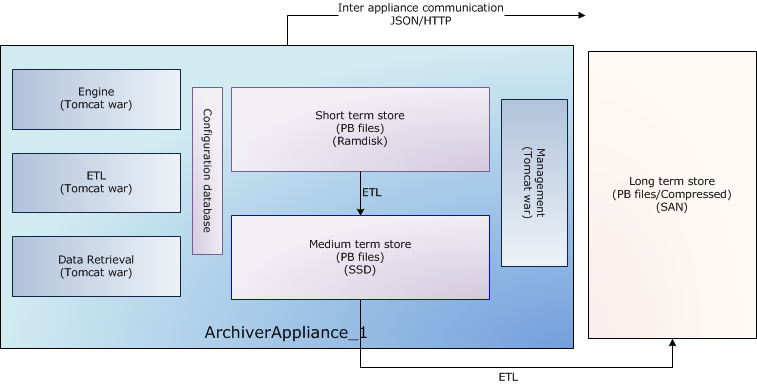
\includegraphics[scale=0.6]{image/applarch}
%     \caption {Modo de funcionamento de uma \textit{appliance}. Extraída de
%     \cite{archiver}.}
%     \label{fig:epics_archiver} 
% \end{figure} 

O instituto desenvolvedor da aplicação sugere que cada módulo seja lançado em
sua própria instância \textit{Tomcat}. Em adição, ele propõe a divisão da
unidade de armazenamento em 3 outras unidades, de acordo com a frequência em que
os dados são salvos. Essas unidades são divididas em \textit{short-term},
\textit{medium-term} e \textit{long-term storage}, cujas frequências de
armazenamento são, respectivamente, a cada hora, diária e anual. Essas
configurações podem ser modificadas através de arquivos
específicos, explicados nas próximas subseções.

\vspace{12pt}


Em um ambiente composto por diversos servidores EPICS e milhares de variáveis a
serem monitoradas, tal como o sistema de controle do \textit{Sirius}, um sistema
capaz de automatizar e agilizar o armazenamento e recuperação de dados se torna
fundamental para o monitoramento de eventuais problemas. Sendo assim, as próximas seções são
dedicadas à instalação e exploração dos recursos disponíveis nesta aplicação.

\subsection {Instalação}

A versão de Junho de 2016 do \textit{archiver} foi instalada no \textit{OPR23},
que se encontra na sala de controle, e pode ser acessada digitando-se o endereço
\texttt{10.0.4.69} em qualquer \textit{browser}. Atualmente, o arquivador possui
36 \textit{PVs} conectadas, contendo, inclusive, algumas das variáveis geradas
pelos receptores GPS, descritos na seção \ref{sec:pvsgps}. As próximas
subseções descrevem algumas das modificações realizadas no \textit{archiver}.

\subsubsection{\textit{Login} necessário}

Um dos principais problemas do arquivador é que qualquer pessoa logada
pode inserir ou remover variáveis do sistema. A fim de impedir que usuários não
autorizados realizem tais ações, modificou-se o código das
\textit{appliances} para verificar se o usuário foi autenticado com sucesso.
Para tal, instalamos um servidor LDAP no OPR23 e criamos uma página
de \textit{login}, acessada a partir de \url{http://10.0.4.69/login.html}. Quando o
usuário aperta o botão \textit{Ok}, uma requisição do tipo \textit{POST} é
enviada ao módulo \textit{PHP} que roda no servidor. Esse módulo consulta o LDAP
e retorna se o usuário foi autenticado ou não. Em caso de sucesso, uma nova
requisição do tipo \textit{POST} é enviada e capturada pelo módulo
\textit{management}, que, em seguida, inicia uma nova sessão para o usuário.
Enfim, antes de qualquer operação de inserção ou remoção de variáveis, o
módulo verifica se a sessão está definida e, caso esteja, autoriza a respectiva
operação. A intenção é integrar este sistema de \textit{login} ao servidor
LDAP do CNPEM no futuro.

\vspace{12pt}

Um usuário, denominado de \textit{Anônimo}, com permissões básicas de leitura é
disponibilizado por padrão e permite que qualquer pessoa consulte o
\textit{archiver} mesmo não estando autenticada.

\subsubsection{Mudanças no estilo}

Alguns arquivos \textit{css} (\textit{Cascading Style Sheet}) foram modificados
para refletir melhor o esquema de cores do laboratório. As imagens do
\textit{logo} também foram modificadas.

\subsection{Uso do CS-Studio no monitoramento} \label{appliance-csstudio}

O \textit{CS-Studio} \cite{css} pode ser usado para monitorar a
\textit{appliance}. Para isso, entre em \texttt{Edit \(>\) Preferences} e acesse
o item \texttt{CSS Applications \(>\) Trends \(>\) Data Browser}. No campo
\textit{Archive Data Server URLs}, adicione o endereço
\url{pbraw://10.0.4.69/lnls-control-archiver}.
Escreva qualquer \textit{Server alias}. Na tabela \textit{Default Archive Data
Sources}, adicione o mesmo endereço e aperte \textit{Ok} para salvar as
alterações.

\vspace{12pt}

É necessário alterar a perspectiva do \textit{CS Studio}. Acesse
\texttt{Windows \(>\) Open Perspective} e escolha \textbf{Data Browser}. Na aba
\textit{Archive Search}, escreva a \textit{URL} configurada anteriormente e no
campo \textit{Pattern}, escreva o nome das variáveis arquivadas que deseja
monitorar. Por exemplo, se escrevermos \texttt{Cnt:MikroE:*}, todas as variáveis
arquivadas para o receptor GPS da seção \ref{sec:pvsgps} poderão ser acessadas.
Clique com o botão direito na variável desejada e acesse \texttt{Process Variable \(>\) Data Browser}.

\subsection{Acessando a \textit{appliance} com \textit{Python}}

A \textit{appliance} pode ser acessada através de requisições \textit{JSON}
realizadas por um módulo escrito em \textit{Python}, por exemplo. Uma interface
gráfica foi implementada, usando os módulos \textit{Qt}, a fim de testarmos a
comunicação. Ela possui um gráfico, onde serão mostrados os dados recuperados,
uma caixa de opções, que possui todas as variáveis arquivadas na
\textit{appliance}, e componentes para seleção das datas de início e fim do
intervalo desejado. A figura \ref{fig:interface} representa o resultado da
implementação.

\vspace{12pt}

% \begin{lstlisting}[language=Python]
% import time
% import urllib2
% import json
% 
% class JsonRequester ():
%     
%     def __init__(self, data_retrieval_url, mgmt_url):
%         self.data_retrieval_url = data_retrieval_url
%         self.mgmt_url = mgmt_url
%     
%     def json_request_variables(self, variables_prefix):
%         
%         url_json = self.mgmt_url + 'bpl/getPVStatus?pv=' + variables_prefix
%         req = urllib2.urlopen(url_json)
%         data = json.load(req)
%         return data
%     
%     def json_request_data(self, variable, from_date, to_date):    
%         
%         retrieval_url = self.data_retrieval_url + "/data/getData.json?"
%         pv_name = ("pv=" + variable).replace(':', '%3A')
%         to_date =   ("&to=" + time.strftime("%Y-%m-%dT%H:%M:%S",to_date) + 
%         				".000Z").replace(':', '%3A')
%         from_date = ("&from=" + time.strftime("%Y-%m-%dT%H:%M:%S",from_date) + 
%         				".000Z").replace(':', '%3A')    
%         url_json = retrieval_url + pv_name + from_date + to_date
%         req = urllib2.urlopen(url_json)
%         data = json.load(req)
%         secs = [x['secs'] for x in data[0]['data']]
%         vals = [x['val'] for x in data[0]['data']]
%         return secs, vals
% \end{lstlisting}
% 
% O método construtor recebe 2 \textit{strings} como parâmetros.
% \textit{data\_retrieval\_url} e \textit{mgmt\_url} estão contidos no arquivo
% \textit{lnls\_appliances.xml} e representam, respectivamente, os endereços dos
% \textit{servlets} de obtenção de dados e gerenciamento da \textit{appliance}. A
% primeira \textit{url} será usada para recuperar os dados e a segunda, para obter
% as informações relativas às variáveis arquivadas.
% 
% \vspace{12pt}
% 
% O método \textit{json\_request\_variables} é responsável por retornar
% informações de uma ou várias variáveis, cujo nome (no caso de uma pesquisa de
% uma única variável) ou prefixo (parte comum ao nome de diversas variáveis) é
% passado como parâmetro. Para tal, utiliza o método \texttt{getPVStatus}, que é
% disponível no \textit{servlet} de gerenciamento e acessível via a \textit{url}
% \texttt{mgmt\_url}. Esse método também recebe como parâmetro nomes ou prefixos
% de variáveis, especificados após o trecho \texttt{pv=} na requisição
% \textit{json}. Para recuperar todas as variáveis arquivadas por uma
% \textit{appliance} que comecem com o prefixo \texttt{MBTemp}, por exemplo,
% bastar utilizarmos \texttt{pv=MBTemp*} na requisição. Uma vez construída a
% \textit{url}, é necessário utilizar as bibliotecas \textit{python}
% \texttt{urllib2} e \texttt{json}, que realizam a comunicação com os
% \textit{servlets}. 
% 
% \vspace{12pt}
% 
% O método \textit{json\_request\_data} retorna os dados arquivados para uma
% determinada variável, passada como parâmetro. Além dela, essa função recebe dois
% outros valores, sendo eles objetos do tipo \textit{time}, cuja implementação
% reside no módulo \texttt{time}. Esses parâmetros representam, por sua vez, as
% fronteiras do intervalo de tempo para o qual se deseja recuperar os dados, sendo
% que \texttt{from\_date} é a data mais antiga e \texttt{to\_date}, a mais
% recente. Se \texttt{to\_date} vale \texttt{None}, então o sistema o interpreta
% como o tempo no qual a chamada da função foi feita. Os dados são recuperados
% através do método \texttt{getData}, disponível no \textit{servlet}
% \texttt{retrieval} da \textit{appliance}. Antes de realizarmos a requisição, é
% necessário traduzir os objetos \textit{time} para o formato aceito pela
% servidor. Sendo assim, utiliza-se o método \texttt{strftime} do módulo
% \texttt{time} que retorna a representação \textit{string}, segundo a máscara
% especificada (no nosso caso, \texttt{\%Y-\%m-\%dT\%H:\%M:\%S}), do objeto
% passado como parâmetro. A requisição é, enfim, realizada através dos mesmos
% métodos que foram usados na função anterior.
% 
% \vspace{12pt}
% 
% O servidor envia todos os dados, isto é, valores e datas do respectivo evento,
% em único vetor de dicionários. Por este motivo, é necessário processarmos essa
% estrutura antes de retorná-la ao programa que chamou o método. Os valores são
% acessíveis pelo índice \texttt{val} e seu tipo depende da aplicação. A data dos
% eventos relativos aos valores são recuperados pelo índice \texttt{secs} e são
% números inteiros que contém o número de segundos desde uma data de referência
% (1 de Janeiro de 1970) usada no \textit{servlet}. É necessário notar que as
% datas retornadas estão em \textit{UTC}, portanto é exigido que tais
% valores sejam convertidos para a o fuso local.
% 
% \vspace{12pt}


\begin{figure}[h]
    
    \centering
    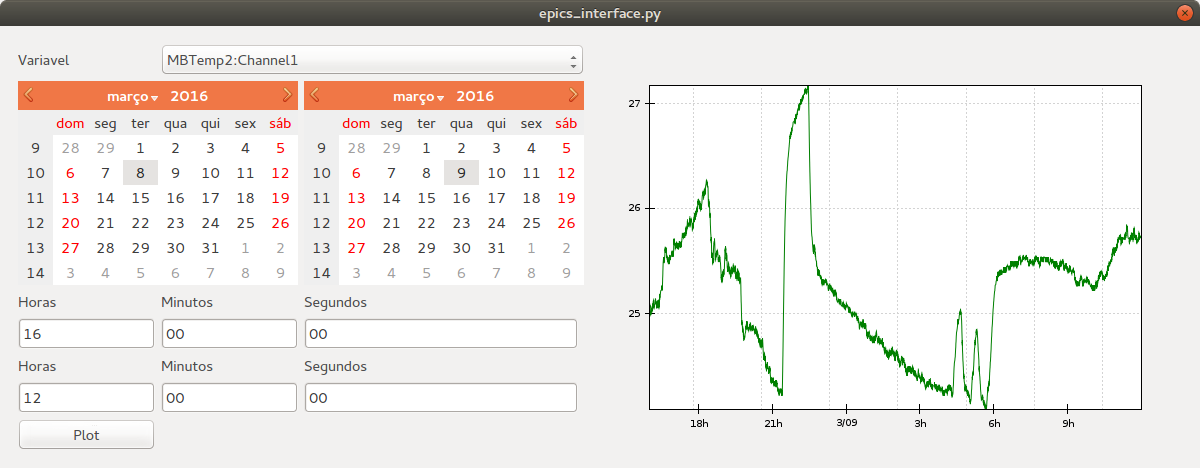
\includegraphics[scale=0.30]{image/screenshot-python}
    \caption {Interface \textit{Qt} implementada em \textit{python}.}
    \label{fig:interface} 
\end{figure} 

\section {Best Ever Alarm System Toolkit - BEAST}

\subsection {Introdução} \label{beast-intro}

Em um ambiente composto por centenas de milhares de variáveis EPICS, como o que
será implementado no \textit{Sirius}, a necessidade de um sistema capaz de
monitorar quais variáveis encontram-se em estados errôneos torna-se
imprescindível. Sendo assim, o monitor de alarmes \textit{BEAST}, do inglês
\textit{Best Ever Alarm System Toolkit} e desenvolvido pelo laboratório
americano \textit{Oak Ridge National Laboratory}, representa uma solução capaz
de gerenciar e controlar os alarmes gerados pelos servidores EPICS disponíveis
na rede. Tal sistema é implementado em \textit{Java} e é baseado no ambiente
gráfico de desenvolvimento \textit{Eclipse}. A arquitetura do sistema
está represetada na figura \ref{fig:best_arquitetura}, logo abaixo.

\FloatBarrier

\begin{figure}[h]

\centering
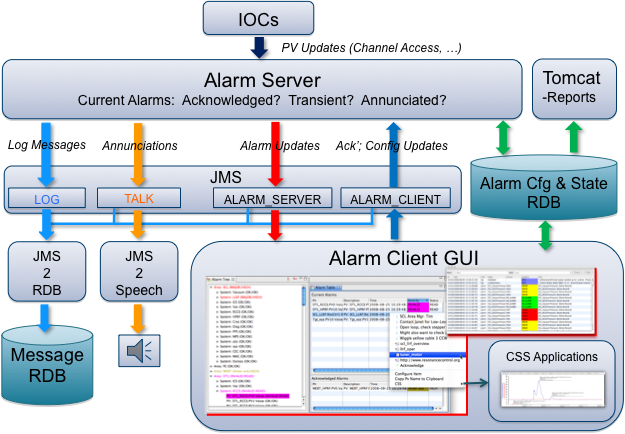
\includegraphics[scale=0.55]{image/beast-arquitetura}
\caption {Implementação do sistema de monitoramento de alarmes
\textit{BEAST}.}
\label{fig:best_arquitetura}
\end{figure}

\FloatBarrier

É possível distinguir diversos componentes na figura acima:

\begin{enumerate}[i.]
  
  \item \textit{Alarm server}: o servidor é responsável por tarefas fundamentais
  no monitoramento de alarmes. Cabe a ele a leitura da configuração dos alarmes
  armazenada no banco de dados \textit{Alarm Cfg \& State RDB}, conectar-se às
  respectivas variávies, monitorar suas mudanças de estado e gerar alarmes
  quando necessário e desativá-los logo que um operador toma conhecimento
  do problema. Esse módulo permite que um número variável de clientes se conecte
  a ele. Uma variável pode adotar duas configurações distintas, sendo elas
  \textit{latch} e \textit{annunciate}. Para a primeira, o servidor mantém o
  alarme de maior gravidade, mesmo que o estado da variável não seja
  atualmente errôneo, até que ele seja reconhecido manualmente pelo operador.
  A fim de impedir um grande volume de alarmes gerados, é possível habilitar
  as opções \textit{delay}, que aciona o alarme somente se o estado errôneo da
  variável se mantiver durante o intervalo de tempo especificado, e
  \textit{count}, que aciona o alarme se tal estado for detectado mais vezes
  que o valor especificado. A segunda configuração ativa o alarme somente
  quando a \textit{PV} apresentar valor inválido, sendo que ele é desativado
  logo que tal variável voltar à sua faixa de operação esperada.
  
  \item \textit{Alarm Cfg \& State RDB}: banco de dados relacional, como um
  servidor \textit{MySQL} por exemplo, onde serão armazenadas as configurações
  de alarme e o atual estado de todos os alarmes.
  
  \item \textit{Java Message Service - JMS}: utilizado para a comunicação entre
  diferentes módulos. No projeto, foi empregada a implementação realizada pelo
  \textit{Apache Software Foundation} chamada de  \textit{Apache ActiveMQ}. O
  sistema utiliza 4 \textit{topics} distintos, sendo eles:
  
  \begin{itemize} \renewcommand\labelitemi{--}
    \item \textit{ALARM\_SERVER}: utilizado pelo servidor para publicar
    atualizações nos estados dos alarmes de acordo com a configuração de cada
    variável.
    
    \item \textit{ALARM\_CLIENT}: permite que clientes notifiquem atualizações
    de configuração e reconhecimento de alarmes.
    
    \item \textit{TALK}: dedicado para anunciar mensagens.
    
  \end{itemize}
  
  \item \textit{Alarm Client GUI}: \label{client-gui} baseado na interface
  gráfica do \textit{Eclipse}, oferece três opções de monitoramento:
  
  \begin{itemize} \renewcommand\labelitemi{--}
    \item \textit{Alarm table}: mostra os alarmes em duas tabelas distintas
    contendo aqueles reconhecidos (\textit{acknowledged alarms}) e aqueles que
    ainda estão acionados (\textit{active alarms}).
    
    \item \textit{Alarm tree}: essa opção de visualização oferece
    uma visão hierarquica dos alarmes, sendo organizada, do nível mais alto para
    o menor, em áreas, sistemas, subsistemas e variáveis. Oferece opções para
    configurar, remover ou adicionar variáveis no nível desejado. O estado do
    alarme de cada item é mostrado por uma cor e por uma anotação, sendo
    composta por três sentenças entre parênteses, que representam
    respectivamente a gravidade atual (\textit{current severity}), a
    maior gravidade detectada anteriormente (\textit{alarm severity}) e o estado
    atual do alarme (\textit{alarm status}). É sincronizada diretamente ao banco
    \textit{Alarm Cfg \& State RDB}, o que implica que uma mudança realizada é
    rapidamente detectada pelo servidor e pelos demais clientes.
    
    \item \textit{Alarm area panel}: indicação gráfica do estado do sistema.
    
  \end{itemize}
  
  É possível, a partir de qualquer uma das \textit{views} presentadas acima,
  acessar outros recursos, como, por exemplo, gráficos e valores atuais das
  variáveis desejadas. Para isso, basta apertar com o botão direito acima da
  \textit{PV} e apertar em \textit{Process variables}.
  
  \vspace{12pt}
  
  A implementação fornece, ainda, suporte para autenticação de usuários via
  \textit{LDAP} ou \textit{JAAS}. Caso seja a escolha, somente usuários
  autorizados podem alterar as configurações de alarmes ou reconhecê-los.
  
  \item \textit{Web reports}: é fornecido também um conteúdo \textit{Web} capaz
  de gerar relatórios, calcular estatísticas (como, por exemplo, totais
  diários, variáveis que mais disparam alarmes, intervalos de tempo que os
  alarmes permanecem mais ativos em média \textit{etc.}) e monitorar os alarmes.
  Assim como os módulos do \textit{EPICS Archiver Appliance}, as páginas devem estar hospedadas em um
  servidor \textit{Tomcat}.
  
\end{enumerate}

\subsection{Instalação}

\textit{BEAST} necessita de uma base de dados relacional, de uma implementação
\textit{JMS} e de um ambiente gráfico baseado no \textit{Eclipse}. Utilizaremos,
respectivamente, o \textit{MySQL}, \textit{Apache ActiveMQ} e a versão
\textit{Eclipse Luna for RCP and Plugin Development}. Uma sugestão de instalação
é apresentada abaixo.

\begin{enumerate}[i.]
  \item  É necessário inicialmente fazer o \textit{download} do
  código fonte do \textit{CS Studio} para obter o produto relacionado ao \textit{Alarm server}.
  Para isso, acesse o repositório do projeto no \textit{GitHub} e extraia os
  arquivos em um diretório. Usaremos aqui o mesmo caminho especificado por
  \texttt{\$INSTALL\_DIR}, utilizado também na seção \ref{sec:archiver}.
  
  \begin{lstlisting}[keywordstyle=\ttfamily, style=nonumbers]
$ cd $INSTALL_DIR/
$ wget https://github.com/ControlSystemStudio/cs-studio/archive/master.zip
$ unzip cs-studio-master.zip
$ rm cs-studio-master.zip
$ cd cs-studio-master/
\end{lstlisting}
   
   Na pasta \texttt{cs-studio-master/}, estão contidos todos os arquivos com os
   códigos-fonte do \textit{CS Studio}, porém só utilizaremos o diretório \texttt{applications/},
   que é o onde está a implementação do \textit{Alarm server}.
   
   \item \label{mysql-alarm} Antes de executar o servidor, é necessário primeiro
   configurar o banco de dados com as tabelas utilizadas por ele. Para isso, diversos
   \textit{scripts} de instalação são disponibilizados pelo desenvolvedor em 
   \texttt{applications/alarm/alarm-plugins/org.csstudio.alarm.beast/dbd}. Vamos
   usar parte do conteúdo contido em \texttt{ALARM\_MYSQL.sql}, uma vez que
   este arquivo adiciona algumas entradas nas tabelas, a fim de testar a
   aplicação. Abra este arquivo e comente as linhas a partir de \texttt{INSERT
   INTO ALARM.ALARM\_TREE VALUES (3, 2, 'System', now());}. As linhas acima
   desta sentença criam a hierarquia, que também nos será útil. Execute, então,
   os seguintes comandos:
   
\begin{lstlisting}[basicstyle=\fontsize{9}{13}\selectfont\ttfamily,
keywordstyle=\ttfamily, style=nonumbers] $ mysql -u root -p
>> CREATE DATABASE ALARM;
>> GRANT ALL ON ALARM.* TO 'lnls_alarm_user'@localhost IDENTIFIED BY 'alarm_password';
>> exit
$ mysql -u lnls_alarm_user -p
>> source applications/alarm/alarm-plugins/org.csstudio.alarm.beast/dbd/ALARM_MYSQL.sql;
\end{lstlisting}

Verifique que as tabelas foram criadas corretamente com:

\begin{lstlisting}[keywordstyle=\ttfamily, style=nonumbers]
>> SHOW TABLES;
\end{lstlisting}
   
\item A próxima etapa é configurar o servidor de mensagens \textit{JMS}. Será
necessário fazer o \textit{download} do pacote \textit{Apache ActiveMQ}.

\begin{lstlisting}[keywordstyle=\ttfamily, style=nonumbers]
$ cd $INSTALL_DIR/
$ wget http://tinyurl.com/htw5tdx
$ tar -xvzf apache-activemq-5.13.0-bin.tar.gz
$ rm apache-activemq-5.13.0-bin.tar.gz
$ cd apache-activemq-5.13.0/
\end{lstlisting}

O diretório \texttt{conf/} contem um arquivo, \texttt{activemq.xml}, com as
configurações do servidor. É possível, por exemplo, modificar a porta, que por
padrão é 61616, ou adicionar autenticação via \textit{jaas}. Para tal, adicione
as seguintes linhas neste arquivo.

\begin{lstlisting}[keywordstyle=\ttfamily, style=nonumbers]
<plugins>
  <jaasAuthenticationPlugin configuration="PropertiesLogin" />
</plugins>
\end{lstlisting}

Neste caso, \textit{PropertiesLogin} é o nome da configuração contido no arquivo
\texttt{login.config}, que especifica os \textit{plugins} necessários e os
arquivos onde estarão armazenados os usuários, suas senhas (\texttt{users.properties}) e grupos
(\texttt{groups.properties}). Por fim, inicie o servidor com 

\begin{lstlisting}[keywordstyle=\ttfamily, style=nonumbers]
$ cd $INSTALL_DIR/apache-activemq-5.13.0/bin/linux-x86-64/
$ ./activemq start
\end{lstlisting}

\item Tendo instalado os componentes responsáveis pela comunicação entre módulos
e base de dados de configurações, podemos iniciar o servidor. Para isso, vamos
utilizar a distribuição \textit{Luna} do \textit{Eclipse for RCP and RAP
Developers}, por apresentar melhor compatibilidade com os pacotes gráficos do
\textit{CS Studio}. Extraia e inicie a aplicação.

\begin{lstlisting}[keywordstyle=\ttfamily, style=nonumbers]
$ cd $INSTALL_DIR/
$ wget http://tinyurl.com/jbmmue7
$ tar -xvzf eclipse-rcp-luna-SR2-linux-gtk-x86_64.tar.gz
$ rm eclipse-rcp-luna-SR2-linux-gtk-x86_64.tar.gz
$ cd eclipse/
$ ./eclipse
\end{lstlisting}

Importe o projeto que contem o servidor de alarmes. Para tal, entre em
\texttt{File > Import \ldots > General > Existing Projects into Workspace} e
escolha o diretório \texttt{\$INSTALL\_DIR/ applications/alarm/}. Dentro deste
projeto, abra o arquivo \texttt{AlamServer.product} contido em
\texttt{alarm-plugins > org.csstudio.alarm.beast.server}. Espera-se que uma tela
parecida com a figura \ref{img:product-view} seja aberta.

\FloatBarrier

\begin{figure}[h]

\centering
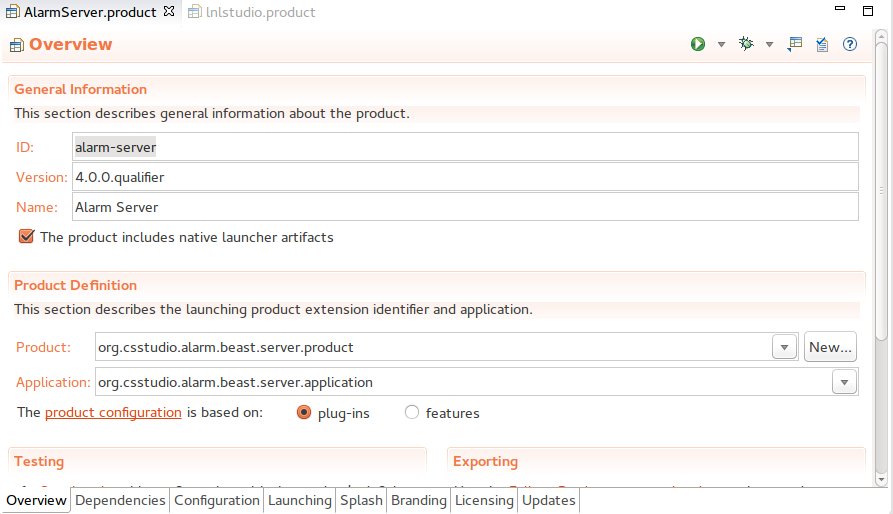
\includegraphics[scale=0.45]{image/product-view}
\caption {Configurações do produto \texttt{AlarmServer.product}.}
\label{img:product-view} 
\end{figure}

\FloatBarrier

Ainda não é possível executá-la, visto que este produto requer algumas
depedências. Para incluí-las à instalação do \textit{Eclipse}, acesse
\texttt{Help > Install New Software\ldots > Add\ldots} e adicione a \textit{url}
\textit{http://download.controlsystemstudio.org/updates/4.1}. Não é necessário
realizar o \textit{download} de todos os pacotes, somente os espeficados na
tabela \ref{tab:plugins} abaixo. A instalação também adiciona os componentes que
permitem o acesso à \textit{appliance}, conforme explicado na seção
\ref{appliance-csstudio}. 

\FloatBarrier
\begin{longtable}[h] {| p{0.3\linewidth} | p{0.3\linewidth} | p{0.3\linewidth}   |}
\caption{\label{tab:plugins} \textit{Plugins} necessários para o
\textit{AlarmServer}.}\\
\hline \multicolumn{3}{| c |}{\textbf{CS-Studio Applications}} \\ \hline
\hline Alarm Handler Tools & Alarm Handler UI & Appliance Archiver Reader (x2) \\ \hline
Application Utilities & Archive Reader RDB Feature & Archive Tools Feature \\ \hline
CS-Studio Epics v3 Support & CS-Studio RAP Utilities & Data Browser \\ \hline
Data Browser OPI Widget & ea4 Archiver Reader & Operator Interface Builder (BOY)\\
\hline \hline \multicolumn{3}{| c|}{\textbf{CS-Studio Core}} \\ \hline \hline
Core Auth Feature & Core Base Feature & Core Platform plugins   \\ \hline
Core Platform RAP Plugins & Core UI Feature & Core Utility Feature \\ \hline
CS-Studio Command-line Execution Services Support & CS-Studio Common Data
Layer (pvmanager) & CS-Studio DAL \\ \hline
CS-Studio Epics v4 Support & CS-Studio Extras Support & PVManager
Autocomplete Featue \\ \hline \hline
\multicolumn{3}{| c|}{\textbf{Maven osgi-bundles}}  \\ \hline \hline
antlr & EPICS Plug-in & Graphene \\ \hline
JSON support for file datasource & JSR 353 API & JSR 353 Default Provider \\ \hline
org.antlr.runtile & org.epics.graphne & org.epics.util \\\hline
org.epics.vtype & org.epics.vtype-json &  org.python.jython \\\hline
pvAccess - Java & pvData - Java &  PVManager Core \\\hline
PVManager EPICS Channel Access Support  & PVManager EPICS PVAccess Support  & 
PVManager Execute Support \\\hline
PVManager File Support  & PVManager Local PV Support  & 
PVManager Simulated PV Support \\\hline
PVManager System Support  & PVManager VType Support  & \\\hline
\end{longtable}
\FloatBarrier

O produto necessita também do \textit{plug-in} \texttt{com.ibm.icu.base} contido
no repositório \textit{Orbit}, acessado através do \textit{link} abaixo.
Selecione somente o pacote \textit{Internacional Components for Unicode for
Java (ICU4J)} e instale-o.

\begin{center}
\textit{http://download.eclipse.org/tools/orbit/downloads/drops/R20150124073747/repository/}
\end{center}

O servidor já pode ser executado, porém ele utilizará uma configuração padrão
para conectar-se ao \textit{MySQL} e ao \textit{JMS}. A fim de modificar tal
configuração, editamos o arquivo \textit{plugin\_ customization.xml}, presente
no mesmo diretório. Esse arquivo deve refletir as instalações realizadas
anteriormente. 

\vspace{12pt}

Entre na aba \texttt{Launching} e adicione o argumento
\texttt{-pluginCustomization} no campo \textit{Program Arguments}. Tal argumento
deve conter o caminho do arquivo \textit{plugin\_customization.xml}, conforme
figura abaixo.

\FloatBarrier

\begin{figure}[h]

\centering
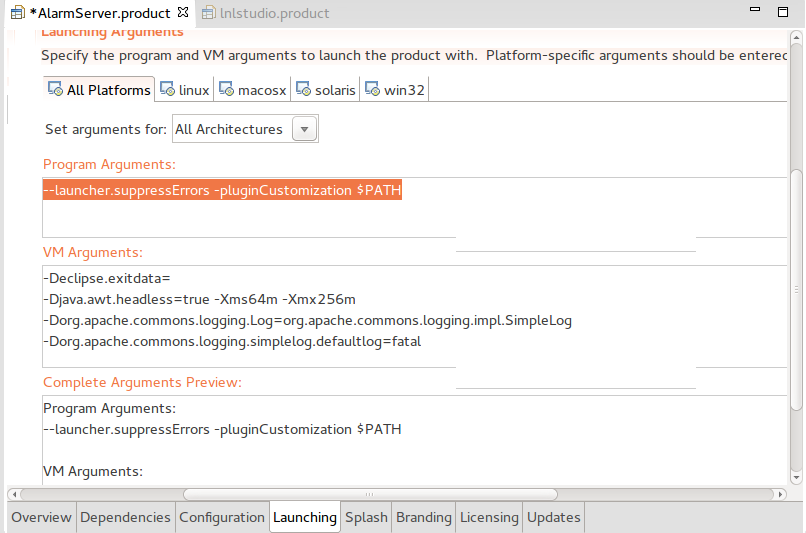
\includegraphics[scale=0.45]{image/launch-view}
\caption {\textit{Launching view} do produto \texttt{AlarmServer.product}.
Substituir \texttt{\$PATH\_TO\_FILE}} pelo caminho completo do arquivo
\textit{plugin\_customization.xml}.
\label{img:launch-view} 
\end{figure}

\FloatBarrier

Execute, enfim, o produto apertando no ícone verde no canto superior direito.
O servidor se encarregará da criação dos \textit{topics} na aplicação
\textit{JMS}. O resultado esperado está representado na figura
\ref{fig:server-on}. \textit{Annunciator} é o nome dado à raíz da hierarquia
criada no item \ref{mysql-alarm} (verificar conteúdo do arquivo
\texttt{ALARM\_MYSQL.sql}) e define, assim, quais tópicos serão utilizados na
comunicação.

\FloatBarrier

\begin{figure}[h]

\centering
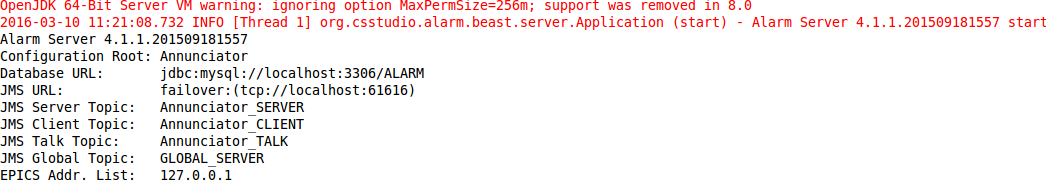
\includegraphics[scale=0.45]{image/alarmserver-on}
\caption {Resultado da execução do produto \textit{AlarmServer}.}
\label{fig:server-on} 
\end{figure}

\FloatBarrier

\end{enumerate}

\subsection{Uso da interface \textit{Eclipse} como \textit{Alarm Client GUI}}

Para configurar o \textit{Eclipse} como um cliente do servidor de alarmes, é
necessário configurá-lo para que ele acesse os servidores \textit{MySQL} e
\textit{JMS}. Isso é realizado através de \texttt{Window > Preferences > CSS
Applications > Alarm > Alarm System}. Modifique os campos\footnote{\textit{RDB}
significa \textit{Relational Database}, como o banco de dados \textit{MySQL}.}
\textit{url}, \textit{username} e \textit{password}, conforme configurado
anteriormente, e reinicie o \textit{Eclipse}. Se tudo foi configurado
corretamente, já é possível acessar os alarmes configurados através do
componentes comentados no item \ref{client-gui} da seção \ref{beast-intro}. Tais
componentes são acessados a partir de \texttt{Window > Show View > Other > CSS}.


\subsubsection {\textit{Debugging}} 

Alguns erros foram encontrados durante a instalação:

\begin{enumerate}[i.]
  \item \textit{A interface não salva corretamente as senhas do banco de dados e
  do JMS}: para resolver este problema basta redefir as senhas que o
  \textit{Eclipse} utiliza para criptografar as senhas salvas. Acesse
  \texttt{Window > Preferences > General > Security > Secure Storage} e redefina
  as senhas contidas na tabela \textit{Master password providers}.

  \item \textit{Não é possível adicionar, remover ou configurar variáveis a
  partir da Alarm Tree View}: conforme explicado na seção \textbf{Introdução}, o
  \textit{BEAST} oferece suporte à autenticação e autorização de usuários. Sendo
  assim, somente usuários cadastrados são permitidos de alterar ou reconhecer
  alarmes. Como a rede do \textit{Sirius} é prevista para ser isolada, tal
  serviço não será necessário. Portanto, podemos configurar o \textit{Eclipse}
  para dar permissão completa a qualquer \textit{user}. Para tal, devemos
  modificar o plugin \texttt{org.csstudio.security}, de extensão \textit{.jar}
  presente no diretório \textit {\$INSTALL\_DIR/eclipse/plugin}. Abra esse
  arquivo com o \textit{Archive Manager} (em sistemas \textit{linux}),
  modifique o campo \texttt{alarm\_config} para \texttt{.*} no arquivo
  \texttt{authorization.conf} e reinicie o \textit{Eclipse}. Deve ser possível
  alterar configurações de alarmes a partir de agora.
\end{enumerate}

\subsubsection {Obtendo um \textit{LNLStudio} a partir da configuração do
\textit{Eclipse}}

É possível exportar a configuração atual do \textit{Eclipse} como um novo
produto, que chamaremos de \textit{LNLStudio}. Para isso, criamos um novo um
novo \textit{Plug-in Project} e adicionamos um novo arquivo do tipo
\textit{Product Configuration}. Neste arquivo, definimos nome, \textit{id},
versão e, no campo \textit{Product Definition}, definimos \textit{Product} como
\texttt{lnlstudio.product} e \textit{Application},
\path{org.eclipse.ui.ide.workbench}. Na aba \textit{Dependencies}, é preciso
especificar quais \textit{plug-ins} são necessários ao produto. Por questão de
simplicidade, adicionamos todos aqueles que estão instalados
(\textit{Add\ldots} e \textit{Ctrl+A} para selecionar todos). Para configurar a
\textit{splash screen}, clique na aba \textit{Splash} e adicione uma
\textit{progress bar}, uma \textit{progress message} e um arquivo chamado
\textit{splash.bmp} ao diretório do projeto. Essa imagem deve possuir dimensões
455x295. 

\vspace{12pt}

O produto pode ser lançado através do ícone verde presente no canto superior da
tela.

\vspace{12pt}

Para exportar este produto, clique em \textit{Eclipse Product export wizard} na
seção \textit{Exporting} da aba \textit{Overview} e escolha o endereço e formato
(arquivo \textit{.zip} ou pasta) para o qual ele deve ser exportado. Para
executar, entre na pasta criada (ou extraída do arquivo) e execute o aplicativo
\texttt{eclipse}.


\section{Conclusao}

\newpage

\bibliographystyle{plain}
\bibliography{references} 

% \section* {Referências bibliográficas}
\begin {itemize}
  \item \url{https://en.wikipedia.org/wiki/Sunspot}. Acessado às 19:22 29/09/2015.
  \item Guyon, I.; Elisseeff, A. "An introduction to variable and feature selection", Journal of Machine Learning Resear ch, vol. 3, pp. 1157 - 1182 2003.
  \item \url{http://archive.ics.uci.edu/ml/datasets/Wine+Quality}.\\
  	 Acessado às 21:27 30/09/2015.
\end{itemize} 

\end{document}
